% Numeração de títulos no CORPO até o terceiro nível (ex.: 7.1.1, 8.1.1.1).
% Sumário enxuto: mostra só capítulos e seções (x.x); as subseções continuam
% numeradas no texto, apenas não aparecem no sumário.
% (Para mostrar as subseções no sumário, troque tocdepth para 2.)
% Idealmente, mover estas linhas para o preâmbulo do documento principal.
\setcounter{secnumdepth}{3}
\setcounter{tocdepth}{1}

\chapter{\label{chap:autotune_contexto}Correção Automática de Afinação Vocal no Contexto da Produção Musical}

Este capítulo apresenta os principais conceitos relacionados à correção automática de afinação vocal no contexto da produção musical. Inicialmente, discute-se o que caracteriza esse tipo de tecnologia e como ela funciona. Em seguida, abordam-se suas aplicações práticas na produção musical, bem como as principais ferramentas comerciais disponíveis. Por fim, discute-se a integração dessas ferramentas com ambientes de produção digital, especialmente as DAWs.

\section{O que é a correção automática de afinação vocal}

A correção automática de afinação vocal, popularmente conhecida como autotune, é um recurso utilizado para ajustar a afinação de uma gravação vocal. Em termos gerais, seu funcionamento envolve identificar a frequência fundamental da voz em determinado instante e, a partir disso, deslocá-la para uma nota alvo previamente definida ou pertencente a uma escala musical \cite{decheveigne2002yin, mauch2014pyin}.

\section{Aplicações na produção musical}

O uso de ferramentas de correção vocal ocorre em diferentes contextos. Em produções mais naturais, o objetivo costuma ser preservar ao máximo a expressividade da interpretação, realizando apenas ajustes discretos de afinação \cite{moulines1990psola}. Já em outras produções, especialmente em gêneros como trap, pop e música eletrônica, a correção vocal pode ser utilizada como elemento estilístico marcante, alterando de forma perceptível o timbre e a transição entre notas \cite{antares_autotune_pro}.

Dessa forma, a correção automática de afinação vocal pode ser entendida não apenas como um mecanismo técnico de correção, mas também como um recurso criativo. Em muitos casos, ela passa a compor a identidade sonora de artistas e músicas, tornando-se parte da estética do gênero musical em que está inserida \cite{antares_autotune_manual}.

Além disso, essas ferramentas normalmente são utilizadas em conjunto com outros recursos de produção, como equalização, compressão, reverberação e efeitos de ambiência. Isso faz com que sua aplicação esteja diretamente relacionada ao ambiente de produção digital no qual a voz é gravada, editada e processada \cite{ableton_manual}.

\section{Ferramentas comerciais e acessibilidade}

Atualmente, existem diversas ferramentas comerciais voltadas à correção automática de afinação vocal. Entre as mais conhecidas, destaca-se o Auto-Tune, da Antares, amplamente utilizado na indústria musical e frequentemente associado ao próprio conceito de correção vocal automática \cite{antares_autotune_pro,antares_autotune_manual}.

A Figura~\ref{fig:antares_autotune} apresenta uma imagem oficial da interface do Auto-Tune Pro, utilizada neste trabalho como referência visual de uma solução comercial consolidada.

\begin{figure}[h]
    \centering
    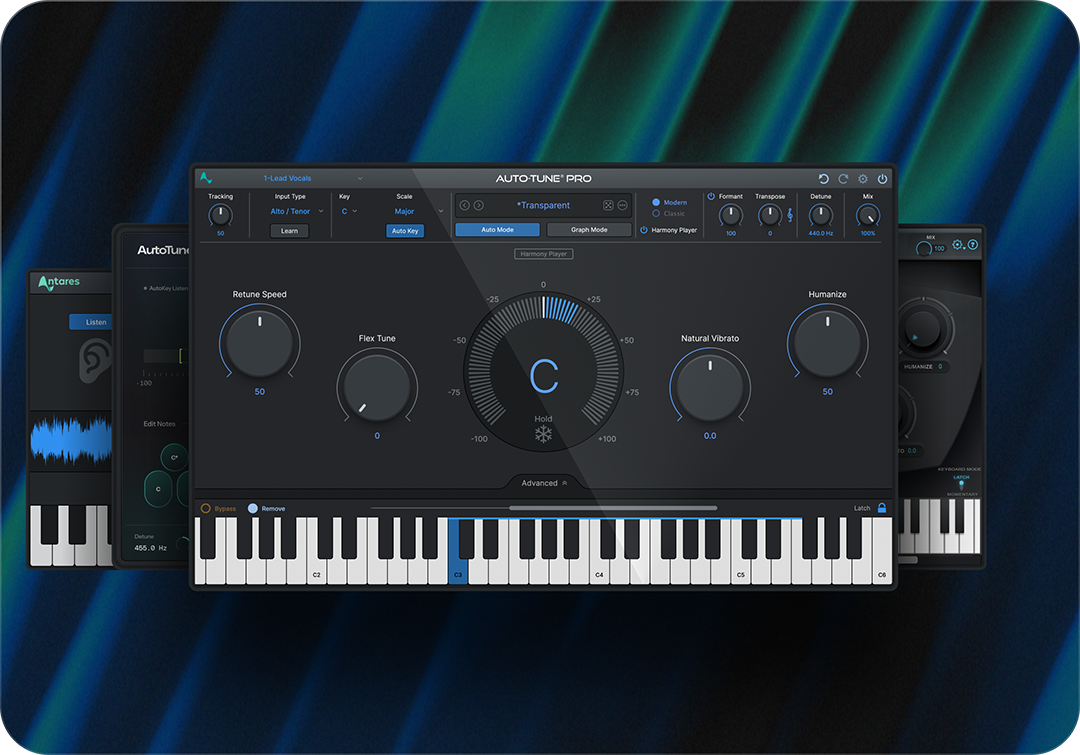
\includegraphics[width=0.9\textwidth]{fig/antares-autotune.png}
    \caption{Interface do usuário do Auto-Tune Pro, da Antares.}
    \label{fig:antares_autotune}
    \small Fonte: Antares Tech \cite{antares_autotune_pro,antares_autotune_manual}.
\end{figure}

Além dele, também existem outras soluções consolidadas no mercado, com diferentes propostas de controle, qualidade de processamento e integração com ambientes de produção musical \cite{ableton_manual}.

Entretanto, muitas dessas ferramentas são pagas e, em vários casos, os recursos mais avançados estão disponíveis apenas em versões de maior custo. Isso pode limitar o acesso de artistas e produtores independentes \cite{antares_autotune_pro}.

\section{DAWs e integração com plugins de áudio}

As ferramentas de correção automática de afinação vocal normalmente são utilizadas dentro de ambientes conhecidos como DAWs, sigla para \textit{Digital Audio Workstations}. Uma DAW é um software voltado à gravação, edição, produção, mixagem e processamento de áudio digital \cite{ableton_manual}.

Entre os exemplos mais conhecidos está o Ableton Live, amplamente utilizado na produção musical contemporânea. A Figura~\ref{fig:ableton_live} apresenta uma imagem oficial da interface do software.

\begin{figure}[h]
    \centering
    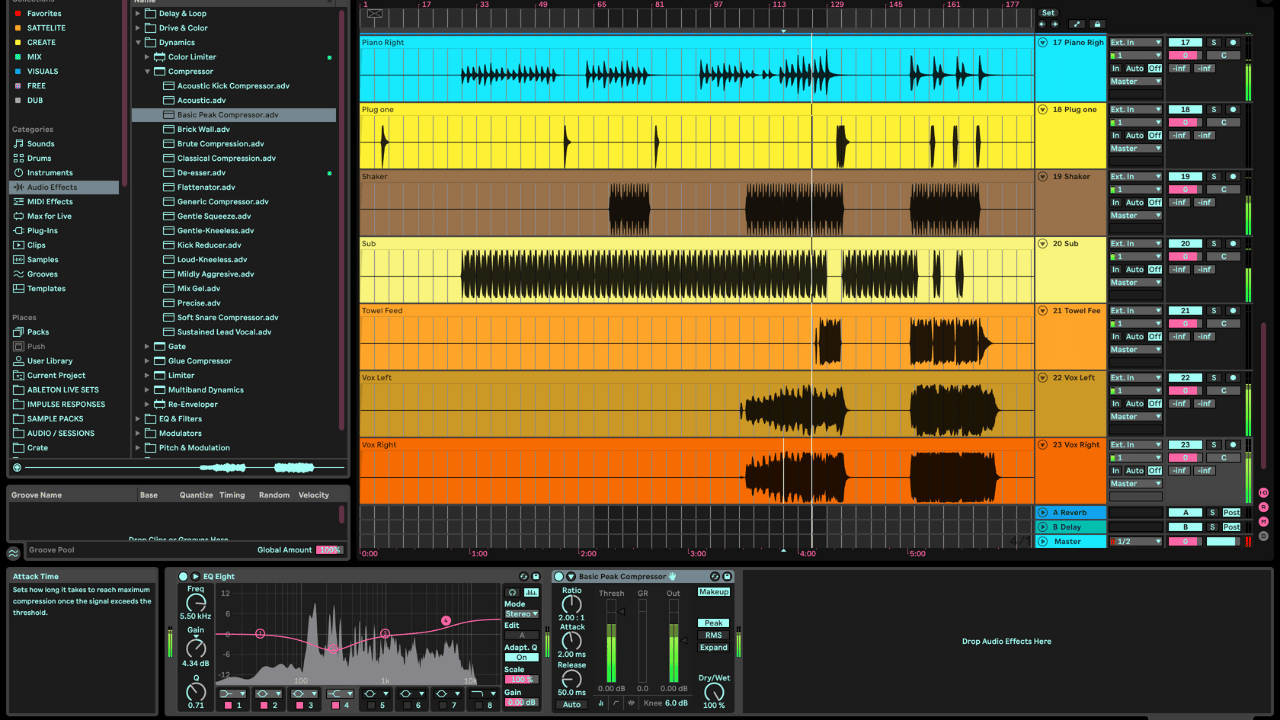
\includegraphics[width=0.8\textwidth]{fig/ableton-live.png}
    \caption{Interface do usuário do Ableton Live.}
    \label{fig:ableton_live}
    \small Fonte: Ableton \cite{ableton_live,ableton_manual}.
\end{figure}

No contexto da produção musical, a DAW pode ser entendida como o ambiente principal de trabalho do produtor musical, reunindo em um único sistema recursos para organizar trilhas, gravar vocais, inserir efeitos e testar diferentes decisões sonoras ao longo de um projeto \cite{ableton_manual}.

Nesse processo, ferramentas de correção de afinação normalmente aparecem como plugins de áudio carregados dentro da DAW. Esses plugins recebem o sinal vocal, processam a informação de pitch e devolvem o áudio corrigido ao projeto musical. Dessa forma, a DAW funciona como plataforma de integração entre gravação, edição e processamento em tempo real ou offline \cite{ableton_manual,antares_autotune_manual}.


\chapter{\label{chap:problema}Problema}

A correção automática de afinação vocal tornou-se uma tecnologia amplamente presente na produção musical, sendo utilizada tanto para corrigir pequenas imprecisões de interpretação quanto para produzir efeitos estéticos característicos em diferentes gêneros musicais. Apesar de sua ampla utilização, a implementação de uma ferramenta desse tipo envolve uma série de desafios técnicos que não são triviais, especialmente quando se busca desenvolver uma solução própria, ainda que apoiada em bibliotecas de software livre \cite{antares_autotune_pro}.

Nesse contexto, o problema central deste trabalho está no desafio de compreender e recriar os mecanismos fundamentais que tornam esse tipo de tecnologia viável na prática. Desenvolver um autotune próprio exige lidar com etapas como a detecção da frequência fundamental da voz, a definição da nota alvo, a lógica de correção e a preocupação com critérios como estabilidade, precisão e potencial de uso com baixa latência \cite{decheveigne2002yin,mauch2014pyin,aalto_speech_properties,aalto_f0_estimation}.

Entre essas etapas, a detecção de pitch ocupa um papel muito importante ao detectar de forma consistente a frequência fundamental presente no sinal vocal. No entanto, essa tarefa é complexa, já que a voz humana não se comporta como um sinal perfeitamente periódico. Em sinais reais, estão presentes ruído, harmônicos, transientes, variações tímbricas e instabilidades naturais de emissão, fatores que dificultam a identificação correta do pitch ao longo do tempo.

Além disso, diferentes algoritmos de detecção de pitch apresentam características distintas em termos de precisão, robustez, estabilidade e custo computacional. Assim, ao buscar recriar uma ferramenta de correção automática de afinação, torna-se importante investigar quais abordagens oferecem uma base mais adequada para sustentar o desenvolvimento do produto final. Nesse sentido, a comparação entre algoritmos como autocorrelação, YIN e pYIN constitui uma etapa essencial para orientar as decisões técnicas do protótipo \cite{delacuadra2007pitch,decheveigne2002yin,mauch2014pyin}.

Dessa forma, o problema deste trabalho consiste em investigar como construir um protótipo experimental de correção automática de afinação vocal, com o apoio de bibliotecas de software livre, utilizando a análise comparativa de algoritmos de detecção de pitch como fundamento para o desenvolvimento da solução final. O foco está em compreender de que maneira essas abordagens podem contribuir para a construção de um sistema que seja tecnicamente consistente e capaz de servir como base para uma ferramenta funcional de autotune.

Assim, mais do que apenas estudar algoritmos isoladamente, este trabalho busca enfrentar um problema prático e técnico de maior escopo: identificar quais mecanismos são mais adequados para viabilizar a recriação de uma tecnologia de correção automática de afinação vocal em um contexto experimental, acessível e academicamente fundamentado.

A questão que orienta este trabalho pode ser expressa da seguinte forma:

\begin{quote}
Como desenvolver, com o apoio de bibliotecas de software livre, um protótipo de correção automática de afinação vocal, e de que forma a comparação entre diferentes algoritmos de detecção de pitch pode contribuir para a construção dessa solução final?
\end{quote}



\chapter{\label{chap:proposta}Proposta}

O objetivo deste trabalho é desenvolver um protótipo experimental de correção automática de afinação vocal, fundamentado na comparação entre diferentes algoritmos de detecção de pitch, de modo a investigar quais abordagens oferecem melhor base técnica para a construção da solução proposta.

Este capítulo apresenta a proposta do trabalho, descrevendo sua visão geral, o levantamento das necessidades do usuário, o escopo definido, os requisitos do protótipo e as etapas previstas para o seu desenvolvimento.

\section{Visão geral da proposta}

Este trabalho propõe o desenvolvimento de um protótipo experimental de correção automática de afinação vocal, com foco na implementação, comparação e avaliação dos principais componentes envolvidos nesse tipo de tecnologia. Entre esses componentes, destaca-se especialmente a etapa de detecção de pitch, uma vez que ela constitui a base para a identificação da frequência fundamental e, consequentemente, para o processo de correção de afinação \cite{aalto_f0}.

A proposta parte do entendimento de que ferramentas de correção vocal ocupam atualmente papel relevante no fluxo de produção musical. Nesse contexto, o trabalho busca investigar, de forma prática, como esse tipo de sistema pode ser construído a partir de técnicas de detecção de pitch, definição de nota alvo e processamento de correção de frequência \cite{antares_autotune_pro, ableton_manual}. 

A proposta não tem como objetivo competir diretamente com soluções comerciais consolidadas, como os plug-ins amplamente utilizados na indústria musical. Em vez disso, busca-se construir uma base técnica e experimental que permita estudar o problema de forma acessível, com ênfase em fins acadêmicos, educacionais e de prototipagem. Assim, o valor principal do trabalho está menos na entrega de um produto comercial completo e mais na construção de um artefato funcional que permita compreender as decisões algorítmicas e de implementação envolvidas na correção automática de afinação vocal.

De maneira geral, o protótipo foi desenvolvido em duas frentes complementares. Na primeira, foi realizado um estudo comparativo entre diferentes algoritmos de detecção de pitch, em ambiente Python, com foco nas abordagens de autocorrelação, YIN e pYIN; ao longo do trabalho, incluiu-se também o SWIPE', como representante de um paradigma espectral distinto dos demais. Na segunda, após a análise comparativa e a escolha da abordagem mais adequada, foi implementada a lógica principal de correção de afinação em C++, com apoio do framework JUCE, evoluindo o sistema até uma primeira versão funcional (MVP) \cite{delacuadra2007pitch,decheveigne2002yin, mauch2014pyin,librosa_pyin_docs, cppreference_cpp, juce_website}.

\section{Levantamento das necessidades do usuário}

Como parte da etapa inicial do trabalho, foi realizada uma conversa com um usuário com experiência prática no uso de ferramentas de correção vocal em contexto de produção musical. O objetivo dessa interação foi compreender como esse tipo de ferramenta é utilizado no fluxo real de gravação e pós-produção, bem como identificar quais características seriam mais relevantes em um protótipo experimental.

De modo geral, o levantamento indicou que a correção de afinação é utilizada principalmente durante a gravação, em tempo real, e posteriormente complementada na pós-produção com ajustes mais finos. Entre os aspectos mais valorizados pelo usuário, destacaram-se a precisão na correção da nota, a naturalidade do resultado sonoro, latência baixa e a facilidade de uso da ferramenta.

Também foram apontados como problemas importantes das soluções atuais a alta complexidade de operação, a falta de naturalidade em determinadas correções e, principalmente, a limitação de algumas ferramentas ao uso em tempo real em razão da latência elevada. Nesse sentido, a baixa latência foi identificada como requisito essencial para que um protótipo possa ser considerado útil em contexto de teste ao vivo.

Além disso, o usuário indicou preferência por definir manualmente a escala ou tonalidade de referência, embora considere desejável a existência de suporte automático de identificação em relação ao instrumental. 

Com base nesse levantamento, foram definidos como requisitos prioritários do protótipo: (i) correção automática de afinação em tempo real; (ii) baixa latência; (iii) precisão na estimação e correção das notas; (iv) preservação de naturalidade sonora; e (v) simplicidade de uso. Esses requisitos ajudam a orientar tanto a comparação entre os algoritmos de detecção de pitch quanto as decisões de implementação do protótipo ao longo do desenvolvimento.

\begin{table}[H]
\centering
\caption{Síntese das necessidades levantadas com o usuário}
\begin{tabular}{|p{5cm}|p{8cm}|}
\hline
\textbf{Aspecto} & \textbf{Necessidade identificada} \\
\hline
Momento de uso & Principalmente em tempo real durante a gravação, com ajustes posteriores na pós-produção \\
\hline
Prioridade principal & Precisão na correção da nota \\
\hline
Qualidade desejada & Naturalidade sonora e bom encaixe no tom da música \\
\hline
Problemas atuais & Alta latência, falta de naturalidade e complexidade de uso \\
\hline
Controles desejados & Correção automática, controle de pitch e controle de naturalidade \\
\hline
Requisito essencial do protótipo & Correção automática em tempo real com baixa latência \\
\hline
\end{tabular}
\small Fonte: Elaborada pelo autor.
\end{table}

\subsection{Comparação com sistemas similares e funcionalidades desejadas}

O protótipo proposto assemelha-se, em seu propósito e em seu fluxo de uso, a
ferramentas de correção vocal já consolidadas no mercado, como o Auto-Tune da
Antares, o Melodyne, o Waves Tune e o GSnap. Todas compartilham o mesmo núcleo
funcional: estimar a frequência fundamental da voz, definir uma nota ou escala de
referência e deslocar a afinação em direção a essa referência, normalmente na forma
de um plugin carregado em uma DAW \cite{antares_autotune_pro,ableton_manual}. Nesse
sentido, o sistema desenvolvido posiciona-se como uma alternativa experimental e de
software livre a essas soluções, com foco acadêmico e educacional.

A partir do levantamento inicial com o usuário, observou-se que, mesmo em
ferramentas consolidadas, alguns aspectos são frequentemente apontados como
limitações: a complexidade de operação de certas ferramentas, a perda de
naturalidade em correções mais intensas, a latência elevada que dificulta o uso em
tempo real e o custo de acesso às versões mais completas. Foi também manifestado o
desejo de que a ferramenta identifique automaticamente a tonalidade do instrumental,
em vez de exigir que a escala seja sempre informada manualmente.

Parte dessas necessidades já foi contemplada no protótipo: a baixa latência foi
tratada como requisito central; a naturalidade é dosável por meio dos parâmetros de
força, tolerância e glide; e a simplicidade norteou o desenho da interface. A
detecção automática de tonalidade, por outro lado, foi identificada como uma
funcionalidade desejável ainda não implementada, sendo viável de incorporar e
prevista como uma das frentes do próximo semestre (Capítulo~\ref{chap:cronograma}).

Cabe registrar que o levantamento realizado nesta etapa teve caráter inicial e
exploratório, baseado em uma entrevista com um usuário experiente. Um estudo com
usuários mais amplo --- com sessões de uso do protótipo, comparação direta com
ferramentas similares e coleta sistemática de feedback --- está previsto para a
etapa seguinte, de modo a validar empiricamente a utilidade do sistema e a orientar
seu refinamento.

\section{Requisitos do protótipo}

Com base no levantamento realizado com o usuário e na análise dos aspectos observados no contexto de uso, os requisitos do protótipo foram organizados em requisitos funcionais e não funcionais. Os requisitos funcionais descrevem as principais capacidades que o sistema deverá oferecer, enquanto os requisitos não funcionais estabelecem características de qualidade e restrições relevantes para o desenvolvimento e para a validação do protótipo.

\subsection{Requisitos funcionais}

\begin{itemize}
    \item RF01: Ler sinais de áudio monofônicos para processamento.
    \item RF02: Estimar a frequência fundamental do sinal de entrada ao longo do tempo.
    \item RF03: Permitir definir uma nota, escala ou tonalidade de referência para a correção.
    \item RF04: Aplicar correção automática de afinação com base na referência definida.
    \item RF05: Permitir ajuste de parâmetros relacionados à intensidade e à naturalidade da correção.
\end{itemize}

\subsection{Requisitos não funcionais}

\begin{itemize}
    \item RNF01: O protótipo deve operar com baixa latência em contexto experimental.
    \item RNF02: O sistema deve apresentar precisão adequada na estimação da frequência fundamental.
    \item RNF03: O resultado da correção deve preservar naturalidade sonora sempre que possível.
    \item RNF04: A implementação deve ser modular, favorecendo testes e futuras extensões.
    \item RNF05: O protótipo deve ser simples de operar em contexto de validação experimental.
\end{itemize}

\section{Escopo do trabalho}

O escopo deste trabalho compreende a investigação e a implementação dos elementos essenciais de uma solução de correção automática de afinação vocal. Entre esses elementos, destacam-se: a leitura e análise de sinais de áudio monofônicos, a estimação da frequência fundamental ao longo do tempo, a definição de uma nota alvo ou de uma escala de referência e a aplicação de uma lógica de correção que aproxime o sinal vocal dessa referência musical \cite{aalto_f0_estimation}.

Como parte do escopo, foi dada atenção especial à etapa de detecção de pitch, uma vez que ela constitui a base para o restante do processamento. Foram comparados diferentes algoritmos com relação a critérios como precisão, estabilidade, comportamento em sinais vocais reais, custo computacional e adequação ao uso pretendido no protótipo. Essa etapa foi importante para fundamentar tecnicamente a escolha da abordagem principal adotada na implementação posterior \cite{delacuadra2007pitch}.

No que se refere especificamente à etapa de correção de afinação, entende-se que se trata de um problema mais amplo e mais complexo, por envolver não apenas a detecção da frequência fundamental, mas também decisões relacionadas à forma de deslocamento do sinal, à preservação de características sonoras e à qualidade perceptiva do resultado final. Em razão dessa complexidade, este trabalho não propôs um estudo sobre os algoritmos de correção de pitch. Em vez disso, foi adotada uma técnica já consolidada na literatura e amplamente utilizada em processamento de voz, a PSOLA (\textit{Pitch-Synchronous Overlap-Add}) --- mais especificamente sua variante no domínio do tempo, a TD-PSOLA ---, como base para a implementação da etapa de correção \cite{moulines1990psola,aalto_psola}.

Também fez parte do escopo o desenvolvimento de versões incrementais do protótipo, cada uma delas destinada a validar parcialmente o fluxo proposto. A submissão dessas versões à apreciação de um usuário com experiência no uso de Ableton Live e Auto-Tune da Antares --- de modo a incorporar feedback qualitativo ao longo da evolução do sistema, e não apenas ao final --- terá continuidade no próximo semestre, conforme o cronograma do Capítulo~\ref{chap:cronograma} \cite{antares_autotune_pro,ableton_live}.

\section{Etapas de desenvolvimento}

O desenvolvimento da proposta foi conduzido de forma incremental. Inicialmente, foi preparada uma base experimental em Python, destinada à implementação e à avaliação dos algoritmos de detecção de pitch selecionados. Essa etapa permitiu trabalhar com maior agilidade na comparação entre abordagens, testar diferentes amostras de áudio e registrar limitações, vantagens e comportamentos observados em cada método \cite{delacuadra2007pitch}.

Em seguida, com base nos resultados obtidos na fase experimental, foi escolhida a abordagem de detecção de pitch mais adequada ao objetivo do protótipo. A partir dessa escolha, foi definido o fluxo principal de processamento, contemplando a sequência geral de operações do sistema: detectar a frequência fundamental do sinal de entrada, identificar a nota ou referência musical desejada e aplicar uma lógica de correção que desloque a afinação do áudio em direção a essa referência.

Na etapa posterior, a implementação principal foi evoluída em C++, utilizando o framework JUCE. Essa escolha se justifica por sua ampla utilização no desenvolvimento de aplicações e plug-ins de áudio, além de sua adequação a cenários que exigem maior controle sobre desempenho, organização do processamento e futura aproximação com contextos reais de produção musical \cite{juce_website,juce_github, cppreference_cpp}. Nessa fase, o objetivo foi transformar os aprendizados obtidos na experimentação em Python em uma arquitetura mais próxima de um protótipo de uso real.

A etapa de correção de afinação foi implementada com base na técnica TD-PSOLA, adotada neste trabalho como solução de referência para o deslocamento de pitch. Essa decisão buscou manter o escopo viável e tecnicamente consistente, concentrando o esforço investigativo principal na comparação entre algoritmos de detecção de pitch e na integração desses resultados a um fluxo funcional de correção vocal \cite{moulines1990psola,aalto_psola}.

Por fim, o trabalho contempla uma etapa contínua de validação dos protótipos desenvolvidos, cuja parte de avaliação com usuário terá continuidade no próximo semestre. Cada versão incremental implementada será testada por um usuário com experiência prática no uso de Ableton Live e Auto-Tune da Antares, com o objetivo de coletar percepções qualitativas sobre o comportamento do sistema, sua coerência com o fluxo real de produção musical e a utilidade das funcionalidades implementadas até aquele estágio. Dessa forma, o desenvolvimento não dependerá apenas de uma validação final, mas incorporará feedback do usuário ao longo da evolução do protótipo, contribuindo para orientar refinamentos sucessivos e fundamentar a análise dos resultados \cite{antares_autotune_pro,ableton_live}.

\chapter{\label{chap:conceitos_basicos}Conceitos Básicos}

Este capítulo apresenta os conceitos fundamentais necessários para a compreensão da proposta. São abordados tópicos relacionados a áudio digital, período, frequência fundamental, pitch, harmônicos e detecção de pitch.

\section{Áudio digital}

O áudio digital pode ser entendido como a representação discreta, em computador, de um sinal sonoro originalmente contínuo no tempo. Esse processo de digitalização ocorre, de forma geral, em duas etapas principais: a amostragem e a quantização. A amostragem consiste em medir a amplitude do sinal em instantes igualmente espaçados no tempo, gerando uma sequência de amostras. Já a quantização consiste em representar a amplitude dessas amostras em um conjunto finito de níveis discretos, definidos pela profundidade de bits utilizada no sistema \cite{digitalsound_digitization}.

Nesse contexto, a taxa de amostragem determina quantas amostras do sinal são coletadas por segundo, enquanto a profundidade de bits determina quantos níveis discretos podem ser usados para representar a amplitude de cada amostra. Esses dois parâmetros afetam diretamente a qualidade da representação digital do som e são fundamentais em qualquer sistema de processamento de áudio \cite{digitalsound_digitization}.

\section{Período, frequência e frequência fundamental}

Em sinais periódicos, o período corresponde ao intervalo de tempo necessário para que um padrão do sinal se repita. A frequência, por sua vez, expressa quantas repetições ocorrem por segundo e é medida em Hertz (Hz). A relação entre essas duas grandezas é dada por:

\begin{equation}
T = \frac{1}{f}
\end{equation}

No contexto de sinais sonoros aproximadamente periódicos, como a voz em trechos vozeados, a frequência fundamental (\(F_0\)) corresponde à frequência associada à estrutura periódica básica do sinal. Em outras palavras, trata-se da taxa média de repetição da oscilação principal observada no som, sendo uma das grandezas centrais para a análise e o processamento de voz e áudio musical \cite{aalto_f0}.

\section{Pitch e harmônicos}

Embora frequentemente relacionados, os conceitos de frequência fundamental e pitch não são exatamente equivalentes. A frequência fundamental descreve uma propriedade física do sinal, enquanto pitch está associado à percepção auditiva dessa frequência pelo ouvinte. Em muitos casos, ambos coincidem de forma aproximada, mas há situações em que o pitch percebido pode não corresponder diretamente à presença física da componente fundamental no espectro \cite{aalto_f0,aalto_speech_properties}.

Em sinais harmônicos, além da componente fundamental, surgem componentes em frequências que são múltiplos inteiros de \(F_0\). Essas componentes são chamadas de harmônicos e podem ser expressas, de forma geral, como:

\begin{equation}
f_k = kF_0, \quad k = 1,2,3,\ldots
\end{equation}

A estrutura harmônica é importante porque influencia fortemente a forma como o som é percebido, contribuindo não apenas para a identificação do pitch, mas também para características tímbricas do sinal. Em voz e em muitos sons musicais, essa organização harmônica desempenha papel central na análise acústica \cite{aalto_speech_properties}.

\section{Detecção de pitch}

A detecção de pitch consiste no processo de estimar, a partir de um sinal de áudio, a frequência fundamental ao longo do tempo. Essa tarefa é especialmente importante em aplicações como análise de voz, síntese, transcrição musical e correção automática de afinação. Em geral, a estimação é feita sobre trechos curtos do sinal, pois tanto a voz quanto outros sinais musicais variam ao longo do tempo \cite{aalto_f0_estimation,decheveigne2002yin}.

A frequência fundamental pode ser observada em diferentes representações do sinal. No domínio do tempo, ela pode ser associada à repetição temporal da forma de onda; na autocorrelação, aparece como um pico no atraso correspondente ao período; e, no espectro, está relacionada à organização harmônica das componentes em frequência \cite{aalto_f0_estimation}. A partir dessas observações, diferentes métodos de detecção de pitch foram desenvolvidos, incluindo abordagens no domínio do tempo, como a autocorrelação, e algoritmos mais robustos, como o YIN e suas extensões \cite{decheveigne2002yin}.

\chapter{\label{chap:algoritmos_pitch}Algoritmos de detecção de pitch}

Este capítulo apresenta os principais algoritmos de detecção de pitch considerados neste trabalho. Foram selecionadas quatro abordagens com diferentes níveis de complexidade e paradigmas distintos: a autocorrelação, o algoritmo YIN, o algoritmo pYIN e o SWIPE'. A análise desses métodos permite comparar desde uma técnica clássica baseada diretamente na periodicidade do sinal, passando por uma abordagem probabilística mais sofisticada voltada a estimativas estáveis da frequência fundamental, até um método de natureza espectral.

\section{Critérios para escolha dos algoritmos}

A seleção dos algoritmos considerados neste trabalho foi orientada por critérios técnicos e práticos relacionados aos objetivos do protótipo proposto. Como o foco da pesquisa está na construção de uma base consistente para um sistema experimental de correção automática de afinação vocal, os métodos escolhidos precisavam permitir comparação relevante sob diferentes perspectivas.

Primeiramente, buscou-se selecionar algoritmos representativos de níveis distintos de complexidade e robustez. A autocorrelação foi incluída por representar uma abordagem clássica e conceitualmente fundamental na detecção de pitch. O algoritmo YIN foi selecionado por introduzir refinamentos importantes sobre abordagens baseadas em autocorrelação, reduzindo ambiguidades e melhorando a estimação da frequência fundamental. Já o pYIN foi escolhido por estender o YIN com uma abordagem probabilística e modelagem temporal, permitindo estimativas mais estáveis e com informação adicional sobre vozeamento. Por fim, o SWIPE' foi incluído por representar um paradigma distinto dos demais --- de natureza espectral ---, o que permite contrastar os métodos baseados em análise temporal com uma abordagem fundamentada na estrutura harmônica do sinal no domínio da frequência.

Dessa forma, a seleção de autocorrelação, YIN, pYIN e SWIPE' busca compor um conjunto comparativo que abrange desde uma técnica mais simples e tradicional, passando por uma abordagem mais robusta e probabilística, até um método de natureza espectral. Essa organização permite observar, de forma progressiva, como diferentes decisões algorítmicas impactam a qualidade da detecção de pitch e sua adequação ao desenvolvimento do protótipo de autotune.

\begin{table}[H]
\centering
\caption{Critérios adotados para a escolha dos algoritmos de detecção de pitch}
\begin{tabular}{|p{4.2cm}|p{9.5cm}|}
\hline
\textbf{Critério} & \textbf{Justificativa no contexto do trabalho} \\
\hline
Relevância teórica & Selecionar algoritmos consolidados e frequentemente citados na literatura de detecção de pitch. \\
\hline
Representatividade técnica & Incluir abordagens com diferentes níveis de complexidade, desde métodos clássicos até extensões probabilísticas. \\
\hline
Precisão da estimação & Verificar a capacidade do algoritmo de estimar corretamente a frequência fundamental em sinais vocais. \\
\hline
Estabilidade temporal & Avaliar a consistência das estimativas ao longo do tempo, reduzindo oscilações e saltos indesejados. \\
\hline
Comportamento em sinais vocais reais & Observar a robustez do método diante de ruído, harmônicos, transientes e variações naturais da voz. \\
\hline
Custo computacional & Considerar a complexidade do algoritmo e sua viabilidade para uso em um protótipo com restrições de desempenho e latência. \\
\hline
Adequação ao protótipo & Verificar o potencial do método para servir como base à etapa posterior de correção automática de afinação. \\
\hline
Viabilidade experimental & Considerar a disponibilidade de referências, documentação e implementações que permitam testes comparativos em ambiente Python. \\
\hline
\end{tabular}
\small Fonte: Elaborada pelo autor.
\end{table}

\section{Comparação entre os algoritmos}

Com base nos critérios definidos, os algoritmos selecionados podem ser comparados quanto à técnica empregada, ao nível de complexidade, às vantagens, às limitações e a adequação ao objetivo do trabalho. Essa comparação é importante porque a escolha do método principal de detecção de pitch não depende apenas de sua formulação teórica, mas também do seu comportamento prático dentro do contexto de um protótipo de correção automática de afinação vocal.

A autocorrelação representa a base conceitual mais simples entre os métodos analisados, sendo útil como referência inicial de comparação. O YIN, por sua vez, introduz mecanismos voltados à redução de erros típicos da autocorrelação, como ambiguidades relacionadas ao período fundamental. Já o pYIN amplia essa abordagem ao incorporar múltiplos candidatos com probabilidades associadas e um modelo temporal para estimar uma sequência mais estável de frequências fundamentais. O SWIPE', por sua vez, parte de um princípio distinto: em vez de medir periodicidade no tempo, compara o espectro de magnitude do sinal com modelos de série harmônica, trazendo ao estudo um representante de abordagem espectral \cite{delacuadra2007pitch, mauch2014pyin, decheveigne2002yin, camacho2008swipe}.

Nesse sentido, a comparação entre os algoritmos não busca apenas identificar qual método apresenta melhor desempenho absoluto, mas qual deles oferece o melhor equilíbrio entre precisão, estabilidade, custo computacional, robustez e adequação ao escopo do protótipo. Também é importante destacar que a escolha realizada nesta etapa não impede que outros algoritmos venham a ser considerados ao longo do desenvolvimento, caso surjam limitações relevantes nos testes ou necessidade de ampliar o estudo comparativo.

\begin{table}[h]
\centering
\small
\caption{Comparação entre os algoritmos de detecção de pitch selecionados}
\begin{tabularx}{\textwidth}{|p{2.1cm}|p{2.2cm}|X|X|p{2.1cm}|p{2.4cm}|}
\hline
\textbf{Algoritmo} & \textbf{Técnica principal} & \textbf{Vantagens} & \textbf{Limitações} & \textbf{Complexidade assintótica aproximada} & \textbf{Adequação ao trabalho} \\
\hline
Autocorr. & Similaridade entre o sinal e versões deslocadas no tempo &
Simplicidade conceitual; fácil interpretação; boa referência inicial para comparação. &
Suscetível a ambiguidades, erros de oitava e influência de variações do sinal. &
\(O(W^2)\) na forma direta; pode ser reduzida com FFT. &
Alta como referência inicial; moderada como candidata principal. \\
\hline
YIN & Função de diferença normalizada, limiar absoluto e interpolação parabólica &
Maior robustez que a autocorrelação; boa precisão; poucos parâmetros; baixa latência. &
Pode sofrer com sinais difíceis e exige ajuste da faixa de frequências. &
\(O(W^2)\) por quadro, na formulação direta. &
Alta como candidata principal para o protótipo. \\
\hline
pYIN & Extensão probabilística do YIN com múltiplos candidatos e modelagem temporal via HMM/Viterbi &
Maior estabilidade temporal; melhor tratamento de ambiguidades; fornece probabilidade de vozeamento. &
Maior complexidade computacional e de parametrização; integração mais custosa. &
Superior à do YIN, pois inclui modelagem temporal. &
Alta para comparação avançada; depende de testes para uso em tempo real. \\
\hline
SWIPE' & Casamento espectral com \textit{kernels} de série harmônica (abordagem espectral) &
Robusto a variações de amplitude; paradigma distinto dos métodos temporais. &
Sensível a ruído e a erros de oitava; sem modelagem temporal; mais custoso por quadro. &
\(O(F \log F)\) pela FFT, mais o casamento dos \textit{kernels} de candidatos. &
Útil como contraste de paradigma (espectral); menos adequado como candidato principal. \\
\hline
\end{tabularx}
\small Fonte: Elaborada pelo autor.
\end{table}

Cabe destacar que as complexidades apresentadas na tabela são aproximadas e têm caráter comparativo, pois dependem da formulação adotada, do tamanho da janela de análise e da implementação utilizada.

\section{\label{sec:autocorrelacao}Autocorrelação}

A autocorrelação é uma das abordagens mais clássicas para a estimação da frequência fundamental (\(F_0\)) em sinais de áudio. Sua ideia central consiste em medir a similaridade entre um sinal e uma versão deslocada de si mesmo no tempo. Quando o sinal apresenta comportamento aproximadamente periódico, como em trechos de voz ou em sons musicais monofônicos, a comparação com atrasos específicos tende a produzir máximos de similaridade, os quais podem ser associados ao período fundamental do sinal \cite{delacuadra2007pitch,decheveigne2002yin}.

De forma geral, se um sinal possui período \(T_0\), espera-se que ele se pareça com ele mesmo quando comparado com uma cópia deslocada de aproximadamente \(T_0\). Assim, ao calcular a autocorrelação para diferentes atrasos, torna-se possível estimar o período fundamental e, a partir dele, a frequência fundamental, dada por:

\begin{equation}
f_0 = \frac{1}{T_0}
\end{equation}

Em sua formulação discreta, essa medida soma, para cada atraso \(\tau\), o produto entre o sinal e sua versão deslocada ao longo de uma janela de \(W\) amostras --- a expressão completa está no Apêndice~\ref{ap:formulas} (Seção~\ref{ap:autocorr_yin}). Em sinais periódicos, essa função tende a apresentar picos em múltiplos do período do sinal, de modo que a busca pelo pico mais relevante pode ser utilizada como base para a estimação de \(F_0\) \cite{decheveigne2002yin}.

Segundo o review de métodos de detecção de pitch utilizado como referência, a autocorrelação procura justamente essa relação de similaridade entre o sinal e sua versão deslocada. O texto também destaca que, para sinais harmônicos, a função de autocorrelação apresenta picos em múltiplos da frequência fundamental, o que explica sua ampla utilização em tarefas de rastreamento de pitch, especialmente em aplicações relacionadas à fala \cite{delacuadra2007pitch}.

Apesar de sua simplicidade conceitual, a autocorrelação apresenta limitações importantes. Conforme discutido por de Cheveigné e Kawahara, a escolha incorreta de picos pode levar a erros na estimação da frequência fundamental, como a seleção de múltiplos ou submúltiplos do período correto. Além disso, variações de amplitude e características espectrais do sinal podem interferir na forma da função de autocorrelação, dificultando a identificação do atraso correspondente ao período real \cite{decheveigne2002yin}.

Outro ponto relevante é o custo computacional. O review de detecção de pitch observa que, dependendo do tamanho da janela, o cálculo direto da autocorrelação pode exigir grande número de operações de multiplicação e soma. Ainda assim, o mesmo texto aponta que existem formas mais eficientes de computá-la por meio da Transformada Rápida de Fourier (FFT), o que torna essa abordagem mais viável em aplicações práticas \cite{delacuadra2007pitch}.

Do ponto de vista prático, uma implementação de autocorrelação está disponível na biblioteca \texttt{librosa}, por meio da função \texttt{librosa.autocorrelate}. A documentação oficial descreve essa rotina como uma autocorrelação com lag limitado (\textit{bounded-lag auto-correlation}), permitindo controlar o atraso máximo considerado no cálculo. Essa função pode ser útil em experimentos iniciais de análise temporal e como bloco básico para comparação com algoritmos mais sofisticados de estimação de pitch \cite{librosa_autocorrelate_docs}.

No contexto deste trabalho, a autocorrelação é relevante por representar uma abordagem fundamental e historicamente importante na detecção de pitch. Sua inclusão permite compreender a base conceitual sobre a qual algoritmos posteriores, como o YIN e o pYIN, introduzem refinamentos para reduzir ambiguidades, melhorar a robustez e aumentar a precisão da estimação da frequência fundamental.


\section{\label{sec:yin}YIN}

O algoritmo YIN é um método de estimação da frequência fundamental (\(F_0\)) proposto por de Cheveigné e Kawahara com o objetivo de reduzir erros comuns observados em abordagens clássicas de detecção de pitch, especialmente aquelas baseadas em autocorrelação. Segundo os autores, o método foi desenvolvido para produzir menos erros do que técnicas já conhecidas, mantendo formulação relativamente simples, baixa latência e poucos parâmetros a serem ajustados \cite{decheveigne2002yin}.

A ideia central do YIN parte da observação de que, em sinais aproximadamente periódicos, como voz e sons musicais monofônicos, o período fundamental pode ser estimado pela repetição temporal do sinal. O artigo apresenta inicialmente a formulação clássica baseada em autocorrelação, na qual picos em determinados atrasos sugerem possíveis períodos do sinal. No entanto, os autores mostram que a autocorrelação simples está sujeita a erros relevantes, como seleção incorreta de harmônicos, influência de variações de amplitude e ambiguidades entre o período real e múltiplos desse período \cite{decheveigne2002yin}.

Para contornar essas limitações, o YIN substitui a busca direta por máximos de autocorrelação por uma função de diferença, que mede, para cada atraso \(\tau\), o grau de dissimilaridade entre o sinal e uma versão deslocada de si mesmo (formulação no Apêndice~\ref{ap:formulas}, Seção~\ref{ap:autocorr_yin}). Valores pequenos dessa função indicam que o sinal se parece com sua versão deslocada, o que sugere a presença de periodicidade compatível com a frequência fundamental. De acordo com os autores, essa reformulação já reduz significativamente a taxa de erro quando comparada ao uso direto da autocorrelação \cite{decheveigne2002yin}.

Em seguida, o algoritmo aplica uma etapa de normalização acumulada, gerando a chamada \textit{cumulative mean normalized difference function}. Essa transformação é importante porque evita que o método escolha incorretamente atrasos muito pequenos e reduz a influência de mínimos espúrios provocados por características espectrais do sinal. Com isso, a função passa a destacar de forma mais confiável o atraso correspondente ao período fundamental \cite{decheveigne2002yin}.

Após a normalização, o YIN adota um critério de limiar absoluto para selecionar a estimativa do período. Em vez de simplesmente escolher o mínimo global da função, o algoritmo busca o primeiro mínimo local cuja profundidade esteja abaixo de um limiar predefinido. Essa estratégia reduz a ocorrência de erros sub-harmônicos, também chamados de erros de oitava em muitos contextos, que surgem quando múltiplos do período fundamental são escolhidos incorretamente como melhor hipótese \cite{decheveigne2002yin}.

Outra etapa importante do método é a interpolação parabólica em torno do mínimo selecionado. Esse refinamento melhora a precisão da estimativa do período quando o valor real não coincide exatamente com um atraso inteiro amostrado. Dessa forma, o YIN consegue obter uma estimativa mais precisa da frequência fundamental sem aumentar excessivamente o custo computacional \cite{decheveigne2002yin}.

No artigo original, os autores descrevem o YIN como a combinação progressiva de seis etapas: autocorrelação, função de diferença, normalização acumulada, limiar absoluto, interpolação parabólica e seleção da melhor estimativa local. Os resultados experimentais apresentados mostram que o método alcança taxas de erro significativamente menores do que algoritmos concorrentes avaliados sobre bases de fala, o que reforça sua importância como referência na estimação de \(F_0\) para voz e música \cite{decheveigne2002yin}.

Do ponto de vista prático, uma implementação amplamente utilizada do algoritmo está disponível na biblioteca \texttt{librosa}, por meio da função \texttt{librosa.yin}. Segundo a documentação oficial, essa função realiza a estimação da frequência fundamental em quadros curtos e sobrepostos do sinal de áudio, calculando primeiro uma função de diferença normalizada e selecionando o primeiro mínimo abaixo do parâmetro \texttt{trough\_threshold}. Em seguida, a estimativa do período é refinada por interpolação parabólica e convertida em frequência \cite{librosa_yin_docs}.

A função \texttt{librosa.yin} exige que sejam definidos valores mínimos e máximos de frequência, por meio dos parâmetros \texttt{fmin} e \texttt{fmax}, além de permitir o ajuste de parâmetros como taxa de amostragem, tamanho do quadro, salto entre quadros e limiar absoluto. A documentação também destaca que a função suporta entrada multicanal e retorna uma série temporal com as frequências fundamentais estimadas em Hertz \cite{librosa_yin_docs}.

No contexto deste trabalho, o YIN é particularmente relevante por representar um método clássico, amplamente consolidado e com boa relação entre precisão, simplicidade e custo computacional. Além disso, sua implementação em \texttt{librosa} facilita a realização de experimentos em Python, permitindo comparações práticas com outras abordagens de detecção de pitch, como o pYIN.


\section{pYIN}
O algoritmo pYIN (\textit{Probabilistic YIN}) é uma extensão probabilística do algoritmo YIN voltada à estimação da frequência fundamental (\(F_0\)) em sinais monofônicos, como voz e instrumentos melódicos. Enquanto o YIN, proposto por de Cheveigné e Kawahara, produz uma única estimativa de frequência fundamental por quadro, o pYIN, proposto por Mauch e Dixon, busca tornar esse processo mais robusto ao preservar múltiplos candidatos de pitch com probabilidades associadas antes da decisão final \cite{decheveigne2002yin,mauch2014pyin}.

A motivação principal do pYIN está em uma limitação importante do YIN tradicional. Como o método original fornece apenas uma hipótese de \(F_0\) por quadro, eventuais erros locais não podem ser recuperados posteriormente por etapas de suavização temporal. Para contornar esse problema, o pYIN modifica a etapa de seleção do YIN e passa a considerar uma distribuição probabilística sobre o parâmetro de limiar, em vez de utilizar apenas um valor fixo. Como resultado, o algoritmo gera um conjunto de candidatos de frequência fundamental com probabilidades associadas, reduzindo a perda de informação causada por decisões locais rígidas \cite{mauch2014pyin}.

O funcionamento do pYIN pode ser entendido em duas etapas principais. Na primeira, o algoritmo segue a estrutura básica do YIN, baseada na análise de periodicidade do sinal, para obter candidatos de \(F_0\). A diferença central está na substituição do limiar absoluto por uma distribuição probabilística de limiares, o que permite manter diferentes hipóteses plausíveis para cada quadro analisado. Na segunda etapa, esses candidatos são utilizados como observações em um Modelo Oculto de Markov (\textit{Hidden Markov Model} -- HMM), e a sequência mais provável de frequências fundamentais é estimada por meio do algoritmo de Viterbi \cite{mauch2014pyin}.

Essa modelagem temporal é uma das principais vantagens do pYIN. Em vez de depender apenas da melhor hipótese instantânea em cada quadro, o método também considera a continuidade temporal da trajetória de pitch. Isso favorece sequências mais suaves e coerentes ao longo do tempo, além de melhorar a separação entre trechos vozeados e não vozeados. Desse modo, o pYIN tende a apresentar maior robustez em situações nas quais o sinal contém ambiguidades locais, ruído ou instabilidades que dificultam a escolha correta da frequência fundamental em cada instante \cite{mauch2014pyin}.

Os resultados experimentais apresentados por Mauch e Dixon indicam que o pYIN supera o YIN convencional em métricas como \textit{recall}, \textit{precision} e \textit{F-measure}, além de apresentar maior robustez a erros de oitava. Os autores também mostram um exemplo qualitativo com voz cantada em que o pYIN mantém uma trilha de pitch mais estável do que o YIN tradicional, evidenciando a contribuição da abordagem probabilística combinada ao rastreamento temporal \cite{mauch2014pyin}.

Do ponto de vista prático, uma implementação amplamente utilizada desse algoritmo está disponível na biblioteca \texttt{librosa}, por meio da função \texttt{librosa.pyin}. De acordo com a documentação oficial, essa função realiza a estimação da frequência fundamental com base no pYIN e retorna três saídas principais: a série temporal de frequências fundamentais estimadas, um vetor booleano indicando se cada quadro é vozeado e a probabilidade de vozeamento de cada quadro \cite{librosa_pyin_docs}.

A função \texttt{librosa.pyin} requer a definição de uma faixa de frequências de interesse por meio dos parâmetros \texttt{fmin} e \texttt{fmax}, além de permitir o ajuste de outros parâmetros relevantes, como taxa de amostragem, tamanho do quadro, salto entre quadros, número de limiares e taxa máxima de transição de pitch. Dessa forma, a implementação disponível em \texttt{librosa} é especialmente útil em contextos experimentais, pois permite aplicar o pYIN diretamente a sinais de áudio em Python, com controle sobre diferentes aspectos do processo de estimação \cite{librosa_pyin_docs}.

No contexto deste trabalho, o pYIN é particularmente relevante por representar uma evolução do YIN em direção a uma abordagem mais robusta e probabilística. Sua utilização permite analisar não apenas a frequência fundamental estimada, mas também informações complementares sobre vozeamento e confiança, o que pode ser útil em aplicações de correção automática de afinação vocal e em experimentos comparativos com outros algoritmos de detecção de pitch.

\section{SWIPE'}

O algoritmo SWIPE' (\textit{Sawtooth Waveform Inspired Pitch Estimator, prime}) foi proposto por Camacho como um estimador de frequência fundamental de caráter espectral, em contraste com as abordagens temporais discutidas nas seções anteriores \cite{camacho2008swipe}. Sua motivação central é explorar diretamente a estrutura harmônica do sinal no domínio da frequência, em vez de inferi-la a partir de propriedades de periodicidade no tempo.

A ideia básica do método consiste em comparar o espectro de magnitude do sinal com um conjunto de \textit{kernels} de referência, cada um associado a um candidato de frequência fundamental. O \textit{kernel} para um candidato $p$ apresenta lóbulos positivos centrados nos harmônicos $k \cdot p$ (com $k = 1, 2, 3, \ldots$), de modo que candidatos cuja série harmônica coincide com os picos do espectro recebem pontuação mais alta. O candidato que maximiza essa correlação ponderada é selecionado como estimativa de $F_0$ para o quadro \cite{camacho2008swipe}.

A versão original do SWIPE' utiliza múltiplas janelas de análise com tamanhos proporcionais ao período de cada candidato, configurando o que os autores chamam de \textit{Pitch-Strength function with Window Sizes proportional to the period} (P²-WSF). Essa formulação melhora a resolução espectral em torno de cada candidato, mas eleva consideravelmente o custo computacional. Implementações simplificadas, denominadas \textit{single-FFT}, substituem essa estratégia por uma única transformada por quadro, com tamanho fixo, mantendo a estrutura geral do método e reduzindo a complexidade \cite{camacho2008swipe}.

Como característica diferencial em relação às abordagens temporais, o SWIPE' tende a ser mais robusto a variações de amplitude e a oferecer menor custo computacional por quadro, em comparação a métodos que executam etapas de inferência probabilística sobre a sequência de candidatos. Em contrapartida, a estimação por quadro isolado, sem modelagem temporal, torna o método mais suscetível a oscilações entre quadros consecutivos, especialmente em sinais reais com transientes, ruído e variações tímbricas. Esse comportamento é analogamente observado no YIN tradicional, que também opera quadro a quadro sem rastreamento temporal explícito \cite{decheveigne2002yin}.

A inclusão do SWIPE' neste trabalho cumpre dois papéis. Primeiro, amplia o estudo comparativo para além das três variantes de análise temporal já selecionadas (autocorrelação, YIN e pYIN), contemplando um paradigma algoritmicamente distinto. Segundo, permite avaliar empiricamente em que medida uma abordagem espectral pode competir, em precisão e estabilidade, com métodos consolidados de análise temporal no contexto específico de uma ferramenta de correção automática de afinação vocal.

Para fins comparativos, foi implementada neste trabalho a variante \textit{single-FFT} do SWIPE', em Python, utilizando as bibliotecas \texttt{NumPy} e \texttt{librosa} --- esta última apenas para o janelamento dos quadros e a geração da grade de tempos, enquanto a transformada de Fourier é calculada com \texttt{numpy.fft}. A implementação opera no domínio da frequência com janela única por quadro, sem inferência temporal adicional, mantendo equivalência arquitetural com os demais métodos comparados em termos de interface de uso e de parâmetros de entrada. Essa opção mantém o foco da comparação no comportamento algorítmico fundamental, preservando a possibilidade de extensão futura para versões mais elaboradas do método.

\chapter{\label{chap:estudo_comparativo}Estudo Comparativo de Algoritmos de Detecção de Pitch}

Este capítulo descreve o estudo comparativo entre os algoritmos selecionados. As quatro seções tratam, respectivamente, dos conjuntos de dados, das métricas, do pipeline experimental e do protocolo de avaliação em tempo real. Os resultados e a escolha do algoritmo são apresentados no Capítulo~\ref{chap:resultados}.

\section{Conjuntos de dados}

Os algoritmos foram avaliados sobre dois conjuntos. O primeiro é um conjunto de sinais sintéticos gerados em código, em que a $F_0$ é conhecida exatamente e serve de gabarito para medir o erro em condições controladas. O segundo é o \textit{Vocadito}, um conjunto público de voz cantada real, com anotações manuais de $F_0$, usado para observar os algoritmos em condições próximas às de uso. Os sintéticos verificam propriedades básicas em sinais ideais; o \textit{Vocadito} expõe os métodos a ruído, articulação e às variações naturais da voz.

\subsection{Sinais sintéticos}
Foram gerados nove sinais em Python, cada um com 2 segundos, $f_s = 22{.}050$ Hz e \textit{hop length} de 512 amostras --- valores próximos aos das implementações de referência adotadas, o que facilita a comparação com a literatura. Para cada sinal, a trajetória de $F_0$ de referência foi obtida analiticamente das próprias equações de síntese. Os sinais cobrem cinco categorias (Tabela~\ref{tab:sinteticos}), dispostas em ordem crescente de dificuldade: da senoide pura, passando por estrutura harmônica e ruído, até pitch que varia no tempo (vibrato e glissando). Essa gradação isola uma propriedade de cada vez.

\begin{table}[H]
\centering
\caption{\label{tab:sinteticos}Sinais sintéticos utilizados na avaliação.}
\small
\begin{tabular}{|p{3.6cm}|p{3.0cm}|p{7.5cm}|}
\hline
\textbf{Categoria} & \textbf{Identificadores} & \textbf{Descrição} \\
\hline
Senoides puras &
\texttt{sine\_220}, \texttt{sine\_440}, \texttt{sine\_880} &
Sinais com apenas a componente fundamental, em três alturas representativas
da faixa vocal (Lá$_3$, Lá$_4$ e Lá$_5$). Permitem verificar a precisão da
estimação em condição ideal. \\
\hline
Sinais harmônicos &
\texttt{harmonic\_220\_5h}, \texttt{harmonic\_440\_5h} &
Sinais compostos pela fundamental somada a cinco harmônicos de amplitude
decrescente ($1/k$). Aproximam-se de timbres vocais e instrumentais,
permitindo avaliar a robustez do algoritmo a estruturas harmônicas
ricas. \\
\hline
Sinais ruidosos &
\texttt{noisy\_440\_snr20}, \texttt{noisy\_440\_snr10} &
Senoide em 440 Hz somada a ruído gaussiano branco, em duas relações
sinal-ruído (20 dB e 10 dB). Permitem avaliar a degradação dos algoritmos
em condições de captação não ideal. \\
\hline
Vibrato &
\texttt{vibrato\_440} &
Senoide em 440 Hz com modulação de frequência em $\pm 50$ cents a uma taxa
de 5 Hz, simulando vibrato vocal natural \cite{sundberg1987science,prame1994vibrato}. Permite avaliar a capacidade dos
algoritmos de acompanhar variações periódicas de pitch dentro de uma única
nota. \\
\hline
Glissando &
\texttt{glissando\_220\_440} &
Varredura linear de frequência de 220 Hz a 440 Hz em 2 segundos,
representando uma oitava de transição contínua. Avalia o comportamento do
algoritmo diante de pitch não estacionário. \\
\hline
\end{tabular}
\small Fonte: Elaborada pelo autor.
\end{table}

\subsection{Vocadito}
O \textit{Vocadito} \cite{bittner2022vocadito} reúne gravações de voz cantada solo anotadas manualmente em $F_0$, notas e letra, sob licença \textit{Creative Commons BY 4.0} e disponíveis no Zenodo \cite{bittner2022vocadito_zenodo}. Foi escolhido por motivos diretos: é voz solo, exatamente o caso de uso de um autotune e tem anotação manual, que serve de referência confiável para o cálculo do erro. A Tabela~\ref{tab:vocadito} resume o conjunto.

\begin{table}[H]
\centering
\caption{\label{tab:vocadito}Características do conjunto \textit{Vocadito}.}
\small
\begin{tabular}{|p{4.5cm}|p{9.5cm}|}
\hline
\textbf{Aspecto} & \textbf{Descrição} \\
\hline
Tipo de conteúdo & Voz cantada solo (excertos de melodias). \\
\hline
Número de gravações & 40 áudios. \\
\hline
Taxa de amostragem & 44{.}100 Hz, monoaural. \\
\hline
Anotações disponíveis & Trajetórias manuais de $F_0$, notas e letra. \\
\hline
Formato das anotações de $F_0$ & Arquivos CSV com pares (tempo, $F_0$ em Hz);
quadros não vozeados são representados por F$_0 = 0$. \\
\hline
Licença & \textit{Creative Commons BY 4.0}. \\
\hline
Origem & Repositório público Zenodo \cite{bittner2022vocadito_zenodo}. \\
\hline
\end{tabular}
\small Fonte: Elaborada pelo autor.
\end{table}

\section{Métricas de avaliação}

Foram usadas seis métricas, divididas em precisão, estabilidade temporal e custo computacional. No experimento de tempo real somam-se a elas a latência mínima e o tempo de processamento por quadro. Todas as métricas de precisão consideram apenas os quadros vozeados da referência, já que em silêncios e consoantes surdas não há $F_0$ definida. As definições seguem o uso corrente na literatura de \textit{Music Information Retrieval} e de extração de melodia \cite{salamon2014melody,raffel2014mir_eval,mauch2014pyin}. A Tabela~\ref{tab:metricas_resumo} resume o conjunto; abaixo ficam apenas as definições que não são óbvias.

\subsection{Precisão}
A \textit{Raw Pitch Accuracy} (RPA) é a fração de quadros vozeados em que o erro fica abaixo de 50 cents, ou seja, meio semitom:

\begin{equation}
\label{eq:rpa}
\text{RPA} \;=\; \frac{1}{|V|} \sum_{i \in V}
\mathbb{1}\!\left( \left| c_{\text{pred}}[i] - c_{\text{ref}}[i] \right| \leq 50 \right),
\end{equation}

\noindent com $V$ o conjunto de quadros vozeados, $\mathbb{1}(\cdot)$ a função indicadora e a conversão para cents dada por $c(f) = 1200 \cdot \log_{2}(f / f_{\text{ref}})$, em que $f_{\text{ref}}$ é uma constante que se cancela na diferença. A \textit{Raw Chroma Accuracy} (RCA) repete a RPA, mas projeta a diferença na classe de altura (\textit{chroma}), ignorando erros de oitava; a distância entre RPA e RCA mede, portanto, quanto dos erros são saltos de oitava. Já a \textit{Gross Pitch Error} (GPE) mede, entre os quadros vozeados em que o algoritmo também emitiu uma estimativa de $F_0$, a proporção daqueles com erro relativo acima de 20\%, isto é, os erros grosseiros:

\begin{equation}
\label{eq:gpe}
\text{GPE} \;=\; \frac{1}{|V_{\star}|} \sum_{i \in V_{\star}}
\mathbb{1}\!\left(
\left| \frac{f_{\text{pred}}[i]}{f_{\text{ref}}[i]} - 1 \right| > 0{,}2
\right).
\end{equation}

\noindent em que $V_{\star} = \{\, i \in V : f_{\text{pred}}[i] > 0 \,\}$ é o subconjunto dos quadros vozeados da referência em que o algoritmo também produziu uma estimativa de pitch. Os quadros em que o algoritmo declara ausência de $F_0$ são, portanto, excluídos do cálculo da GPE --- diferentemente da RPA, em que tais quadros contam como erro.

\subsection{Estabilidade temporal}
Precisão média não basta. A etapa seguinte de \textit{pitch shifting} amplifica qualquer tremor entre quadros, que acaba virando artefato audível. Esse tremor é medido pelo desvio-padrão das variações de $F_0$ de um quadro para o outro, em cents:

\begin{equation}
\label{eq:estab}
\sigma_{\text{estab}}
\;=\; \mathrm{std}\!\Big(\, c_{\text{pred}}[i] - c_{\text{pred}}[i-1] \,\Big)_{i \in V'},
\end{equation}

\noindent com $V'$ os pares de quadros vozeados consecutivos. Quanto menor, mais suave a trajetória. A medição em cents mantém a escala perceptual: o mesmo desvio relativo pesa igual em qualquer região do espectro.

\subsection{Custo computacional}
São duas medidas: o tempo médio por arquivo, dado pela média de execuções repetidas, e o pico de memória, obtido com o módulo \texttt{tracemalloc} da biblioteca padrão do Python. Nenhuma é perceptual, mas ambas pesam na decisão sobre uso em tempo real.

\subsection{Métricas de tempo real}
A latência mínima é o atraso entre o usuário emitir o som e a primeira estimativa de $F_0$ aparecer. Ela vem de duas parcelas: o tempo para encher um quadro de análise (\textit{frame buffer}) e o atraso do filtro de suavização (\textit{look-ahead}):

\begin{equation}
\label{eq:latencia}
L \;=\; \underbrace{\frac{N_{\text{frame}}}{f_s}}_{\text{frame buffer}}
\;+\;
\underbrace{\frac{N_{\text{look}} \cdot N_{\text{hop}}}{f_s}}_{\text{look-ahead do suavizador}},
\end{equation}

\noindent com $N_{\text{frame}}$ o tamanho do quadro, $N_{\text{hop}}$ o salto entre quadros, $N_{\text{look}}$ os quadros futuros que o filtro consulta e $f_s$ a taxa de amostragem; filtros causais têm $N_{\text{look}} = 0$. Estudos de latência em áudio interativo situam o limite tolerável para monitoração ao vivo na ordem de algumas dezenas de milissegundos \cite{lagokon2004}, faixa coerente com a prática de produção em ferramentas comerciais de correção vocal \cite{antares_autotune_pro,ableton_manual}; adota-se aqui o teto de 20 a 30~ms. O tempo de processamento por quadro, $T_{\text{frame}}$, precisa caber no intervalo entre dois quadros:

\begin{equation}
\label{eq:tempo_real_viavel}
T_{\text{frame}} \;<\; \frac{N_{\text{hop}}}{f_s}.
\end{equation}

\noindent Quando essa condição falha, o atraso se acumula e o tempo real deixa de ser possível.

\begin{table}[H]
\centering
\caption{\label{tab:metricas_resumo}Síntese das métricas adotadas.}
\small
\begin{tabular}{|p{3.2cm}|p{2.6cm}|p{6.6cm}|p{1.6cm}|}
\hline
\textbf{Métrica} & \textbf{Categoria} & \textbf{Interpretação} & \textbf{Sentido} \\
\hline
RPA & Precisão & Proporção de quadros com erro $\leq 50$ cents. & Maior $\uparrow$ \\
\hline
RCA & Precisão (sem oitava) & Igual à RPA, projetando a diferença na classe de altura. & Maior $\uparrow$ \\
\hline
GPE & Precisão (erros grosseiros) & Proporção de quadros com erro relativo $> 20\%$. & Menor $\downarrow$ \\
\hline
$\sigma_{\text{estab}}$ & Estabilidade & Desvio-padrão das diferenças quadro a quadro em cents. & Menor $\downarrow$ \\
\hline
Tempo (s) & Custo & Tempo médio de execução por arquivo. & Menor $\downarrow$ \\
\hline
Memória (MB) & Custo & Pico de memória alocada na execução. & Menor $\downarrow$ \\
\hline
Latência (ms) & Tempo real & Atraso até a primeira estimativa em \textit{streaming}. & Menor $\downarrow$ \\
\hline
$T_{\text{frame}}$ (ms) & Tempo real & Tempo de CPU para processar um quadro. & Menor $\downarrow$ \\
\hline
\end{tabular}
\small Fonte: Elaborada pelo autor.
\end{table}

\section{Pipeline experimental}
\label{sec:pipeline_experimental}

O pipeline que roda em Python é o mesmo para todos os algoritmos, apenas a função de detecção que muda. Assim, qualquer diferença nas métricas vem do algoritmo, e não do resto do processo. Para cada par (sinal, algoritmo), ele lê o sinal e a referência, executa o algoritmo (gerando a $F_0$ estimada e o vozeamento), alinha estimativa e referência na mesma grade, calcula as métricas sobre os quadros, mede o custo em uma execução isolada e grava tudo em CSV. A consolidação em tabelas e figuras é feita depois, para não precisar reprocessar os sinais a cada análise.

\subsection{Parâmetros comuns}
 Todos os algoritmos usaram a mesma configuração (Tabela~\ref{tab:parametros_pipeline}), de modo que diferenças de janelamento ou de faixa de frequências não contaminassem a comparação. A faixa $[65, 1000]$ Hz vai do grave das vozes masculinas ao agudo das femininas \cite{aalto_speech_properties} e, de quebra, reduz erros de oitava ao encurtar o espaço de busca. No experimento de tempo real (Seção~\ref{sec:benchmark_realtime}), $f_{\text{min}}$ é reajustado conforme o tamanho do quadro.

\begin{table}[H]
\centering
\caption{\label{tab:parametros_pipeline}Parâmetros comuns adotados no pipeline experimental.}
\small
\begin{tabular}{|p{4.0cm}|p{3.5cm}|p{7.0cm}|}
\hline
\textbf{Parâmetro} & \textbf{Valor} & \textbf{Observações} \\
\hline
Taxa de amostragem $f_s$ &
22{.}050 Hz (sintéticos); 44{.}100 Hz (\textit{Vocadito}) &
Mantida na resolução original de cada conjunto; sem reamostramento. \\
\hline
\textit{Frame length} $N_{\text{frame}}$ & 2048 amostras &
Valor padrão das implementações de referência. \\
\hline
\textit{Hop length} $N_{\text{hop}}$ & 512 amostras &
75\% de sobreposição entre quadros consecutivos. \\
\hline
$f_{\text{min}}$ / $f_{\text{max}}$ & 65 Hz / 1000 Hz &
Cobre da região grave masculina (Dó$_2$) ao agudo feminino (acima de Si$_5$). \\
\hline
Janela de análise & Hann &
Aplicada nos algoritmos que operam no domínio da frequência. \\
\hline
\end{tabular}
\small Fonte: Elaborada pelo autor.
\end{table}

\subsection{Alinhamento e custo}
Como cada algoritmo entrega a $F_0$ em sua própria grade temporal e a referência do \textit{Vocadito} está em outra resolução, a referência é reamostrada por interpolação linear sobre a grade do algoritmo, e o vozeamento, pelo vizinho mais próximo, para não criar rótulos intermediários (a expressão da interpolação está no Apêndice~\ref{ap:formulas}, Seção~\ref{ap:alinhamento}). As duas trajetórias são então cortadas no menor comprimento comum, o que não altera as métricas. O custo é medido à parte, em execução isolada (três repetições nos sintéticos, uma no \textit{Vocadito}), com o pico de memória via \texttt{tracemalloc}. Para garantir reprodutibilidade, a geração dos sinais usa semente fixa, os três métodos temporais vêm das funções \texttt{librosa.autocorrelate}, \texttt{librosa.yin} e \texttt{librosa.pyin} \cite{librosa_autocorrelate_docs,librosa_yin_docs,librosa_pyin_docs} e as versões das bibliotecas estão travadas no projeto. O pipeline inteiro roda de ponta a ponta com um único comando.

\section{Suavização e benchmark em tempo real}
\label{sec:benchmark_realtime}

Até aqui os algoritmos foram tratados como caixa-preta sobre o sinal inteiro. O uso real, porém, é em tempo real: o algoritmo precisa responder quadro a quadro, dentro de um teto apertado de latência. Esse cenário pede três decisões a mais --- suavizar a trajetória bruta, varrer tamanhos de quadro e medir o tempo gasto por quadro ---, descritas a seguir.

\subsection{Por que suavizar}
Mesmo um algoritmo preciso oscila um pouco de um quadro para o outro. Offline, isso é só um $\sigma_{\text{estab}}$ maior; em tempo real, o \textit{pitch shifting} transforma essa oscilação em artefato audível. A suavização entra como um filtro aplicado depois do algoritmo, sem mexer na lógica dele. Todos os filtros trabalham em cents, e não em Hertz, para respeitar a percepção: $\pm 2$~Hz valem $\approx 35$ cents em 100~Hz (audível), mas só $\approx 3{,}5$ cents em 1000~Hz (inaudível).

\subsection{Filtros avaliados}
Foram testados três tipos (Tabela~\ref{tab:smoothers}). A mediana causal ($k = 3, 5$) usa só o passado e não acrescenta atraso. A mediana centrada ($k = 3, 5$) olha quadros futuros e, por isso, custa $\lfloor (k-1)/2 \rfloor$ quadros de \textit{look-ahead}. A média móvel exponencial (EMA) é recursiva e causal:

\begin{equation}
\label{eq:ema}
y[i] \;=\; \alpha \cdot c[i] \;+\; (1 - \alpha) \cdot y[i-1].
\end{equation}

  \noindent Diante desses três filtros de suavização, optou-se pela EMA com $\alpha = 0{,}3$, que atenua o tremor de estimação entre quadros sem introduzir atraso. A preservação de variações musicais lentas, como o vibrato vocal (tipicamente 5--7~Hz \cite{prame1994vibrato}), é assegurada principalmente pela tolerância (zona morta), e não pelo filtro de suavização. A condição sem filtro (\textit{none}) serve de linha de base.

\begin{table}[H]
\centering
\caption{\label{tab:smoothers}Filtros de suavização avaliados.}
\small
\begin{tabular}{|p{4.2cm}|p{4.5cm}|p{2.5cm}|p{2.8cm}|}
\hline
\textbf{Identificador} & \textbf{Tipo} & \textbf{Janela / $\alpha$} & \textbf{\textit{Look-ahead}} \\
\hline
\texttt{none} & --- (linha de base) & --- & 0 quadros \\
\hline
\texttt{median3\_causal} & Mediana causal & $k = 3$ & 0 quadros \\
\hline
\texttt{median5\_causal} & Mediana causal & $k = 5$ & 0 quadros \\
\hline
\texttt{median3\_centered} & Mediana centrada & $k = 3$ & 1 quadro \\
\hline
\texttt{median5\_centered} & Mediana centrada & $k = 5$ & 2 quadros \\
\hline
\texttt{ema\_a0.3} & EMA & $\alpha = 0{,}3$ & 0 quadros \\
\hline
\end{tabular}
\small Fonte: Elaborada pelo autor.
\end{table}

\subsection{Tamanho do quadro}
O tamanho do quadro $N_{\text{frame}}$ é o que mais afeta o uso em tempo real, porque mexe ao mesmo tempo na latência (Eq.~\ref{eq:latencia}), na resolução em frequência e na menor frequência detectável ($f_{\text{min}} \geq f_s / N_{\text{frame}}$). Foram testados os valores 512, 1024 e 2048 amostras. Quando 65 Hz não cabe no quadro escolhido, $f_{\text{min}}$ sobe para o menor valor admissível, $\max(65,\, f_s/N_{\text{frame}} + \epsilon)$, e esse ajuste fica registrado nos resultados.

\subsection{Protocolo}
O benchmark roda todas as combinações de algoritmo, tamanho de quadro e suavizador sobre três gravações do \textit{Vocadito}, em $f_s = 44{.}100$~Hz e $N_{\text{hop}} = 256$. Para cada par (algoritmo, $N_{\text{frame}}$), o algoritmo é executado três vezes e $T_{\text{frame}}$ é a mediana dos tempos por quadro; a $F_0$ bruta é alinhada à referência; cada suavizador é aplicado e calculam-se $\sigma_{\text{estab}}$, RPA e GPE; e a latência sai da Eq.~\ref{eq:latencia}. São seis suavizadores, três tamanhos de quadro e quatro algoritmos, num total de 72 combinações por gravação (216 no conjunto das três gravações). A lista final é ordenada por latência e, em caso de empate, por estabilidade: o que estoura a latência é descartado antes de a precisão entrar em jogo. O ranking resultante, restrito às combinações que cabem no orçamento de latência, é apresentado na Tabela~\ref{tab:realtime_top5} (Seção~\ref{sec:resultados}).


\chapter{\label{chap:resultados}Resultados e Discussão}

  \section{Resultados}
  \label{sec:resultados}

  Esta seção apresenta os resultados obtidos nas três frentes de avaliação: nos
  sinais sintéticos (Seção~\ref{sec:resultados_sinteticos}), no conjunto
  \textit{Vocadito} (Seção~\ref{sec:resultados_vocadito}) e no benchmark em
  tempo real (Seção~\ref{sec:resultados_realtime}). A análise integrada e a
  escolha do algoritmo principal a ser adotado no protótipo são discutidas
  separadamente na Seção~\ref{sec:discussao}.

  \subsection{Sinais sintéticos}
  \label{sec:resultados_sinteticos}

  A Tabela~\ref{tab:resultados_sinteticos} apresenta as métricas obtidas pelos
  quatro algoritmos sobre o conjunto de sinais sintéticos descrito na
  Tabela~\ref{tab:sinteticos}. Os valores correspondem à média e ao desvio-padrão sobre os
  nove sinais avaliados.

  \begin{table}[H]
  \centering
  \caption{\label{tab:resultados_sinteticos}Resultados agregados sobre os sinais sintéticos. Os valores são apresentados como média $\pm$ desvio-padrão sobre os nove sinais. As setas indicam o sentido
  desejado: $\uparrow$ maior é melhor; $\downarrow$ menor é melhor.}
  \resizebox{\textwidth}{!}{%
  \begin{tabular}{|l|c|c|c|c|c|c|}
  \hline
  \textbf{Algoritmo} &
  \textbf{RPA $\uparrow$} &
  \textbf{RCA $\uparrow$} &
  \textbf{GPE $\downarrow$} &
  \textbf{$\sigma_{\text{estab}}$ (cents) $\downarrow$} &
  \textbf{Tempo (s) $\downarrow$} &
  \textbf{Mem (MB) $\downarrow$} \\
  \hline
  autocorr & $1{,}000 \pm 0{,}000$ & $1{,}000 \pm 0{,}000$ & $0{,}000 \pm 0{,}000$ & $5{,}14 \pm 7{,}97$  & $0{,}008 \pm 0{,}001$ & $0{,}83 \pm 0{,}00$ \\
  \hline
  yin      & $0{,}999 \pm 0{,}004$ & $1{,}000 \pm 0{,}000$ & $0{,}001 \pm 0{,}004$ & $22{,}96 \pm 56{,}76$ & $0{,}004 \pm 0{,}000$ & $3{,}58 \pm 0{,}00$ \\
  \hline
  pyin     & $1{,}000 \pm 0{,}000$ & $1{,}000 \pm 0{,}000$ & $0{,}000 \pm 0{,}000$ & $3{,}19 \pm 5{,}51$  & $0{,}203 \pm 0{,}003$ & $23{,}24 \pm 0{,}00$ \\
  \hline
  swipe    & $0{,}888 \pm 0{,}212$ & $0{,}888 \pm 0{,}212$ & $0{,}000 \pm 0{,}000$ & $24{,}84 \pm 38{,}83$ & $0{,}533 \pm 0{,}008$ & $10{,}88 \pm 0{,}00$ \\
  \hline
  \end{tabular}%
  }
  \small Fonte: Elaborada pelo autor.
\end{table}

  \subsubsection{Comportamento nos sinais limpos}

  Nos sete sinais sem ruído (senoides puras, sinais harmônicos, vibrato e
  glissando), os quatro algoritmos atingiram RPA igual a 1{,}000, indicando que
  todos identificaram corretamente a frequência fundamental dentro da tolerância
  de meio semitom. O resultado confirma a correção da implementação dos
  quatro métodos em condições ideais e converge com o comportamento esperado a
  partir de suas formulações teóricas (Capítulo~\ref{chap:algoritmos_pitch}).

  Para o sinal de glissando, em particular, todos os algoritmos foram capazes
  de acompanhar a variação contínua de uma oitava em dois segundos sem
  apresentar erros de oitava ou perda de vozeamento. Para o sinal de vibrato, o
  mesmo padrão se confirmou: as oscilações periódicas de $\pm 50$ cents em
  torno de 440 Hz foram acompanhadas dentro da tolerância da métrica.

  \subsubsection{Comportamento nos sinais ruidosos}

  A presença de ruído gaussiano branco produziu o único caso de degradação
  significativa observado nos sinais sintéticos, e essa degradação se manifestou
  de forma marcadamente assimétrica entre os algoritmos. Os métodos baseados em
  análise temporal — autocorrelação, YIN e pYIN — mantiveram RPA superior a
  $0{,}98$ mesmo na condição mais adversa avaliada (SNR de 10~dB). O SWIPE',
  único método espectral do conjunto, apresentou queda expressiva de desempenho: na decomposição por condição de ruído, não detalhada na tabela agregada, registrou RPA de $0{,}598$ em SNR de 20~dB e $0{,}402$ em SNR de 10~dB, sendo a fonte principal do desvio-padrão elevado observado na agregação
  ($\pm 0{,}212$).

  O contraste é coerente com a natureza dos dois paradigmas. Métodos
  baseados em periodicidade no tempo exploram a estrutura repetitiva do sinal,
  que se preserva razoavelmente sob ruído aditivo independente. Métodos
  espectrais, em contraste, dependem da identificação de picos discretos no
  espectro de magnitude, cuja relação sinal-ruído se deteriora linearmente com
  a degradação do sinal. No caso particular de uma senoide pura ruidosa, a
  ausência de harmônicos reais elimina a vantagem que o SWIPE' obteria em
  sinais harmônicos por meio da soma cruzada entre múltiplos parciais — o que
  explica que o cenário seja especialmente desfavorável para esse método.

  \subsubsection{Estabilidade temporal}

  Em termos de estabilidade temporal, o pYIN apresentou o menor valor médio
  ($\sigma_{\text{estab}} = 3{,}19$ cents), seguido pela autocorrelação
  ($5{,}14$ cents) e, em patamar substancialmente superior, pelo YIN
  ($22{,}96$ cents) e pelo SWIPE' ($24{,}84$ cents). A vantagem do pYIN é
  consistente com a presença da etapa de rastreamento temporal via
  \textit{Hidden Markov Model} discutida no Capítulo~\ref{chap:algoritmos_pitch}: a continuidade imposta
  entre quadros consecutivos suaviza pequenas oscilações que persistem em
  métodos sem modelagem temporal explícita.

  Os desvios-padrão elevados observados em $\sigma_{\text{estab}}$ para YIN
  ($\pm 56{,}76$) e SWIPE' ($\pm 38{,}83$) refletem a heterogeneidade entre os
  sinais: nos sinais limpos a estabilidade é da ordem de unidades de cents,
  enquanto nos sinais ruidosos cresce em uma ordem de magnitude, puxando a
  média e ampliando o desvio.

  \subsubsection{Custo computacional}

  O ordenamento dos algoritmos por custo computacional é nítido. O YIN foi o
  mais rápido ($0{,}004$~s por arquivo de 2 segundos), seguido pela
  autocorrelação ($0{,}008$~s). O pYIN apresentou custo aproximadamente uma
  ordem de magnitude superior ($0{,}203$~s), atribuível ao passo adicional de
  inferência probabilística via algoritmo de Viterbi. O SWIPE', em sua
  implementação \textit{single-FFT} adotada neste trabalho, foi o método mais
  custoso ($0{,}533$~s), em razão da multiplicação matricial entre o conjunto
  de \textit{kernels} de candidatos e o espectro de cada quadro.

  Em termos de pico de memória, a autocorrelação foi a mais econômica
  ($0{,}83$~MB), seguida pelo YIN ($3{,}58$~MB), SWIPE' ($10{,}88$~MB) e
  pYIN ($23{,}24$~MB). A memória adicional consumida pelo pYIN está
  relacionada à manutenção da matriz de transições do modelo probabilístico
  ao longo de todo o sinal.

  \subsubsection{Síntese parcial}

  Nos sinais sintéticos, em condições ideais ou próximas do ideal, os quatro
  algoritmos são equivalentes em precisão. As diferenças aparecem em outros
  eixos: na robustez a ruído os métodos temporais superam claramente o SWIPE'
  espectral; na estabilidade temporal o pYIN se destaca por incorporar
  modelagem entre quadros; e no custo computacional YIN e autocorrelação ficam
  uma ordem de magnitude abaixo de pYIN e SWIPE'. Os próximos resultados
  reavaliam esses padrões sob sinais reais e sob restrições de tempo real.

    \subsection{Vocadito}
  \label{sec:resultados_vocadito}

  A Tabela~\ref{tab:resultados_vocadito} apresenta os resultados obtidos pelos
  quatro algoritmos sobre as 40 gravações do conjunto \textit{Vocadito}. Os
  valores correspondem à média e ao desvio-padrão calculados sobre todas as
  gravações.

  \begin{table}[H]
  \centering
  \caption{\label{tab:resultados_vocadito}Resultados agregados sobre o conjunto \textit{Vocadito}. Os valores são apresentados como média $\pm$ desvio-padrão sobre as 40
  gravações. As setas indicam o sentido desejado: $\uparrow$ maior é melhor; $\downarrow$ menor é melhor.}
  \resizebox{\textwidth}{!}{%
  \begin{tabular}{|l|c|c|c|c|c|c|}
  \hline
  \textbf{Algoritmo} &
  \textbf{RPA $\uparrow$} &
  \textbf{RCA $\uparrow$} &
  \textbf{GPE $\downarrow$} &
  \textbf{$\sigma_{\text{estab}}$ (cents) $\downarrow$} &
  \textbf{Tempo (s) $\downarrow$} &
  \textbf{Mem (MB) $\downarrow$} \\
  \hline
  autocorr & $0{,}983 \pm 0{,}019$ & $0{,}989 \pm 0{,}014$ & $0{,}010 \pm 0{,}017$ & $332{,}92 \pm 113{,}21$ & $0{,}142 \pm 0{,}052$ & $13{,}92 \pm 4{,}88$ \\
  \hline
  yin      & $0{,}977 \pm 0{,}032$ & $0{,}987 \pm 0{,}010$ & $0{,}013 \pm 0{,}032$ & $671{,}58 \pm 147{,}23$ & $0{,}103 \pm 0{,}041$ & $72{,}21 \pm 25{,}61$ \\
  \hline
  pyin     & $0{,}983 \pm 0{,}016$ & $0{,}984 \pm 0{,}012$ & $0{,}001 \pm 0{,}007$ & $29{,}43 \pm 6{,}09$    & $3{,}150 \pm 1{,}199$ & $82{,}50 \pm 21{,}95$ \\
  \hline
  swipe    & $0{,}863 \pm 0{,}151$ & $0{,}879 \pm 0{,}129$ & $0{,}121 \pm 0{,}151$ & $581{,}06 \pm 147{,}55$ & $1{,}266 \pm 0{,}105$ & $23{,}96 \pm 4{,}88$ \\
  \hline
  \end{tabular}%
   }
  \small Fonte: Elaborada pelo autor.
\end{table}

  \subsubsection{Precisão sobre voz real}

  Sob voz cantada real, os três algoritmos baseados em análise temporal
  mantiveram RPA acima de $0{,}97$, com diferenças entre si dentro da margem de
  desvio-padrão observada: autocorrelação ($0{,}983$), YIN ($0{,}977$) e pYIN
  ($0{,}983$). Esse resultado confirma que os três métodos são igualmente
  adequados, em termos de precisão média, para a tarefa de estimação de $F_0$
  em sinais vocais reais. A proximidade entre RPA e RCA, em todos os três
  casos, indica ainda que a quase totalidade dos erros remanescentes ocorre
  dentro da mesma classe de altura, sem trocas de oitava.

  O SWIPE' apresentou comportamento distinto, com RPA de $0{,}863$ e GPE de
  $0{,}121$. A diferença entre RPA ($0{,}863$) e RCA ($0{,}879$) revela que
  apenas uma pequena parte dos erros do SWIPE' corresponde a trocas de oitava: a
  projeção da diferença na classe de altura recupera somente cerca de 1{,}6
  ponto percentual da precisão. Os demais erros grosseiros que compõem o GPE
  elevado ($0{,}121$), portanto, não são saltos de oitava, mas desvios
  grosseiros de outra natureza.
  Esse comportamento é compatível com a variante \textit{single-FFT}
  implementada neste trabalho, que não inclui lóbulos negativos nas posições
  sub-harmônicas do \textit{kernel} de candidatos. A ausência desses lóbulos
  torna o método susceptível a casar parcialmente o espectro com candidatos em
  $p/2$ ou $2p$ do valor correto, especialmente em sinais com estrutura
  harmônica densa, como é o caso da voz cantada.

  \subsubsection{Estabilidade temporal}

  A diferença mais expressiva entre os algoritmos no \textit{Vocadito}
  manifesta-se na estabilidade temporal. O pYIN apresentou
  $\sigma_{\text{estab}} = 29{,}43$ cents, valor uma ordem de magnitude
  inferior aos dos demais métodos: autocorrelação ($332{,}92$ cents), YIN
  ($671{,}58$ cents) e SWIPE' ($581{,}06$ cents). Esses valores correspondem,
  em magnitude perceptual, a oscilações da ordem de semitons completos entre
  quadros consecutivos para os métodos sem modelagem temporal. Um teste de Wilcoxon pareado sobre as 40 gravações confirma que a vantagem do pYIN em estabilidade é estatisticamente significativa em relação a todos os demais métodos ($p < 0{,}001$).

  Esse contraste com os sinais sintéticos
  (Tabela~\ref{tab:resultados_sinteticos}), em que YIN e SWIPE' apresentaram
  $\sigma_{\text{estab}}$ da ordem de poucas dezenas de cents, tem origem no
  material: senoides têm uma fundamental estável em todo quadro, mas a voz real
  traz transientes, articulações e ruído de captação que geram ambiguidades
  locais. Sem continuidade temporal, isso vira decisão oscilante --- e o pYIN é
  o único método avaliado que impõe essa continuidade nativamente, via algoritmo
  de Viterbi.

  Daí a necessidade da etapa de suavização avaliada na
  Seção~\ref{sec:benchmark_realtime}: para os métodos sem modelagem temporal
  embutida, a aplicação de um filtro adequado sobre a trajetória bruta é uma
  condição necessária para a viabilidade em uma aplicação de
  \textit{pitch shifting}.

  \subsubsection{Custo computacional sob sinais mais longos}

  O ordenamento dos algoritmos por tempo total de execução nos sinais reais é o
  mesmo observado nos sintéticos, mas com diferenças absolutas distintas em
  razão da maior duração média dos arquivos. O YIN foi o mais rápido
  ($0{,}103$~s), seguido por autocorrelação ($0{,}142$~s), SWIPE' ($1{,}266$~s)
  e pYIN ($3{,}150$~s). A posição relativamente favorável do SWIPE' em relação
  ao pYIN, em contraste com o observado nos sinais sintéticos, decorre da
  estrutura linear do método: o custo do SWIPE' cresce proporcionalmente ao
  número de quadros, enquanto o pYIN apresenta sobrecargas adicionais
  associadas à inferência temporal sobre sequências mais longas.

  Quanto ao pico de memória, a autocorrelação manteve-se como o método mais
  econômico ($13{,}92$~MB), seguida por SWIPE' ($23{,}96$~MB), YIN
  ($72{,}21$~MB) e pYIN ($82{,}50$~MB). Os valores notavelmente mais elevados
  do YIN e do pYIN sobre o \textit{Vocadito}, em comparação aos sinais
  sintéticos, refletem o maior tamanho dos sinais analisados e o consequente
  crescimento das estruturas internas mantidas durante o processamento.

  \subsubsection{Síntese parcial}

  Os resultados sobre o \textit{Vocadito} apontam na mesma direção em três
  frentes. Em precisão média, autocorrelação, YIN e pYIN têm desempenho
  comparável e adequado à tarefa, enquanto o SWIPE' exibe limitação estrutural
  associada a erros de oitava. Em estabilidade temporal, o pYIN leva vantagem
  expressiva sobre os demais, evidenciando o peso da modelagem temporal
  embutida. Em custo computacional, mantém-se a hierarquia dos sintéticos: YIN
  e autocorrelação baratos, pYIN caro e SWIPE' intermediário no contexto
  \textit{offline} aqui avaliado.

  Precisão equivalente entre os métodos temporais, instabilidade marcante dos
  que não modelam o tempo e custo extra do pYIN: é esse o compromisso que
  motiva a avaliação em tempo real da Seção~\ref{sec:resultados_realtime}.

  \subsection{Benchmark em tempo real}
  \label{sec:resultados_realtime}

  A avaliação em tempo real combina três variáveis: o tamanho do quadro
  ($N_{\text{frame}} \in \{512, 1024, 2048\}$), o filtro de suavização aplicado
  (seis opções, incluindo a linha de base \texttt{none}) e o algoritmo de
  detecção. Os resultados são apresentados em duas tabelas complementares: a
  Tabela~\ref{tab:realtime_resumo} sintetiza, para cada combinação de algoritmo
  e tamanho de quadro, os indicadores observados sob o filtro EMA com
  $\alpha = 0{,}3$, adotado como referência por sua latência adicional nula; a
  Tabela~\ref{tab:realtime_top5} apresenta as cinco melhores combinações dentro
  do orçamento de latência de 30~ms, ordenadas por estabilidade crescente.

  \begin{table}[H]
  \centering
  \caption{\label{tab:realtime_resumo}Resultados em tempo real por algoritmo e tamanho de quadro, sob suavização EMA com $\alpha = 0{,}3$. A latência total inclui o
  \textit{frame buffer} (filtro causal, sem \textit{look-ahead}).}
  \small
  \begin{tabular}{|l|c|c|c|c|c|}
  \hline
  \textbf{Algoritmo} & \textbf{$N_{\text{frame}}$} &
  \textbf{Latência (ms) $\downarrow$} & \textbf{$T_{\text{frame}}$ (ms) $\downarrow$} &
  \textbf{$\sigma_{\text{estab}}$ (cents) $\downarrow$} & \textbf{RPA $\uparrow$} \\
  \hline
  autocorr & 512  & 11{,}61 & 0{,}0255 & 142{,}69 & 0{,}028 \\
  \hline
  autocorr & 1024 & 23{,}22 & 0{,}0323 & 124{,}91 & 0{,}834 \\
  \hline
  autocorr & 2048 & 46{,}44 & 0{,}0466 & 92{,}99  & 0{,}895 \\
  \hline
  yin      & 512  & 11{,}61 & 0{,}0167 & 169{,}84 & 0{,}814 \\
  \hline
  yin      & 1024 & 23{,}22 & 0{,}0344 & 137{,}04 & 0{,}878 \\
  \hline
  yin      & 2048 & 46{,}44 & 0{,}0585 & 137{,}22 & 0{,}911 \\
  \hline
  pyin     & 512  & 11{,}61 & 1{,}3223 & 13{,}13  & 0{,}815 \\
  \hline
  pyin     & 1024 & 23{,}22 & 1{,}7083 & 12{,}78  & 0{,}916 \\
  \hline
  pyin     & 2048 & 46{,}44 & 1{,}7402 & 14{,}45  & 0{,}929 \\
  \hline
  swipe    & 512  & 11{,}61 & 0{,}1441 & 262{,}59 & 0{,}008 \\
  \hline
  swipe    & 1024 & 23{,}22 & 0{,}1948 & 156{,}01 & 0{,}326 \\
  \hline
  swipe    & 2048 & 46{,}44 & 0{,}2769 & 153{,}03 & 0{,}721 \\
  \hline
  \end{tabular}
  \small Fonte: Elaborada pelo autor.
\end{table}

  \begin{table}[H]
  \centering
  \caption{\label{tab:realtime_top5}Cinco melhores combinações com latência total $\leq 30$~ms, ordenadas por estabilidade crescente.}
  \small
  \begin{tabular}{|c|l|c|l|c|c|c|}
  \hline
  \textbf{\#} & \textbf{Algoritmo} & \textbf{$N_{\text{frame}}$} & \textbf{Suavizador} &
  \textbf{Latência (ms)} & \textbf{$\sigma_{\text{estab}}$ (cents)} & \textbf{RPA} \\
  \hline
  1 & pyin & 1024 & \texttt{ema\_a0.3}          & 23{,}22 & 12{,}78 & 0{,}916 \\
  \hline
  2 & pyin & 512  & \texttt{ema\_a0.3}          & 11{,}61 & 13{,}13 & 0{,}815 \\
  \hline
  3 & pyin & 512  & \texttt{median5\_centered}  & 23{,}22 & 15{,}38 & 0{,}858 \\
  \hline
  4 & pyin & 512  & \texttt{median5\_causal}    & 11{,}61 & 16{,}23 & 0{,}817 \\
  \hline
  5 & pyin & 1024 & \texttt{median5\_causal}    & 23{,}22 & 16{,}30 & 0{,}926 \\
  \hline
  \end{tabular}
  \small Fonte: Elaborada pelo autor.
\end{table}

  \subsubsection{Impacto do tamanho do quadro}

  A latência total observada cresce de forma esperada com $N_{\text{frame}}$,
  passando de $11{,}61$~ms em $N_{\text{frame}} = 512$ a $46{,}44$~ms em
  $N_{\text{frame}} = 2048$. Apenas as configurações com $N_{\text{frame}} \in
  \{512, 1024\}$ respeitam o teto prático de 30~ms para uso em tempo real,
  restringindo o espaço de combinações viáveis a duas terças partes do
  universo avaliado.

  O tamanho do quadro também afeta a precisão de forma marcante. Para o pYIN, a
  RPA cresce de $0{,}815$ em $N_{\text{frame}} = 512$ para $0{,}916$ em
  $N_{\text{frame}} = 1024$ e $0{,}929$ em $N_{\text{frame}} = 2048$ —
  incremento atribuível à maior resolução em frequência disponível para o
  algoritmo. Esse mesmo padrão repete-se para os demais métodos. Vale
  registrar que a autocorrelação também colapsa em $N_{\text{frame}} = 512$
  (RPA $= 0{,}028$), ao contrário do YIN no mesmo quadro ($0{,}814$); esse
  comportamento reflete a sensibilidade da implementação de autocorrelação de
  lag limitado adotada a quadros curtos, e uma caracterização detalhada da
  causa foge ao escopo deste experimento, ficando registrada como limitação. O
  caso extremo aparece no SWIPE': em $N_{\text{frame}} = 512$, a resolução de bin
  de aproximadamente $86$~Hz é insuficiente para sustentar a construção dos
  \textit{kernels} de candidatos, reduzindo a RPA a valores próximos de zero
  ($0{,}008$); apenas em $N_{\text{frame}} = 2048$ o método recupera RPA
  acima de $0{,}7$, ainda inferior à dos métodos temporais.

  \subsubsection{Impacto do suavizador na estabilidade}

  A aplicação dos filtros de suavização produz redução substancial de
  $\sigma_{\text{estab}}$ em todos os métodos sem modelagem temporal embutida.
  Para os algoritmos baseados em análise de período, mesmo as configurações
  mais favoráveis avaliadas (suavização causal de mediana com janela $k = 5$ ou
  EMA com $\alpha = 0{,}3$) reduzem o tremor, mas mantêm-no na ordem de
  centenas de cents quando $N_{\text{frame}}$ é pequeno. Para o pYIN, em
  contraste, a estabilidade já é próxima do limiar perceptual de discriminação
  de frequência \cite{moore2012hearing} mesmo antes da
  suavização ($\sigma_{\text{estab}}$ entre 13 e 17 cents nas configurações
  viáveis), e a aplicação do filtro produz refinamento marginal.

  Confirma-se aqui o que já se via nos resultados sobre o
  \textit{Vocadito}: a modelagem temporal embutida no pYIN é, por si só,
  mais eficaz do que qualquer filtro pós-processador avaliado, e os filtros
  externos atuam como compensação parcial para os métodos que não a possuem.

  \subsubsection{Tempo de processamento por quadro}

  A condição de viabilidade em tempo real expressa pela
  Equação~\ref{eq:tempo_real_viavel} ($T_{\text{frame}} < N_{\text{hop}}/f_s$)
  estabelece, para $N_{\text{hop}} = 256$ e $f_s = 44{.}100$~Hz, um limite
  máximo de aproximadamente $5{,}8$~ms por quadro. Todas as combinações
  avaliadas atendem confortavelmente a esse limite, com margens de pelo menos
  três ordens de magnitude para autocorrelação e YIN, duas ordens de magnitude
  para SWIPE' e ainda uma margem confortável (entre $1{,}3$ e $1{,}7$~ms por
  quadro) para o pYIN. Assim, ainda que o pYIN seja o mais caro entre os
  algoritmos avaliados, seu custo permanece compatível com a operação em tempo
  real nas configurações testadas.

  \subsubsection{Síntese parcial}

  A análise integrada da Tabela~\ref{tab:realtime_resumo} e da
  Tabela~\ref{tab:realtime_top5} revela um padrão claro: as cinco melhores
  combinações dentro do orçamento de 30~ms pertencem todas ao pYIN. Os métodos
  baseados em análise temporal sem modelagem entre quadros (autocorrelação e
  YIN) apresentam estabilidade insuficiente para uso direto, mesmo com
  suavização agressiva. O SWIPE', em sua variante \textit{single-FFT}, não
  alcança simultaneamente latência aceitável, estabilidade compatível e
  precisão adequada em nenhuma das configurações avaliadas. A discussão e a escolha do algoritmo principal, na
  Seção~\ref{sec:discussao}, partem desse padrão.

  \section{Discussão e escolha do algoritmo}
  \label{sec:discussao}

  A discussão integrada dos resultados das Seções~\ref{sec:resultados_sinteticos},~\ref{sec:resultados_vocadito} e~\ref{sec:resultados_realtime}
  organiza-se em torno de três observações principais e culmina na escolha do
  algoritmo a ser adotado no protótipo.

  \subsection{Precisão média não discrimina os métodos temporais}

  Em condições ideais (sinais sintéticos limpos), os quatro algoritmos
  apresentam precisão equivalente. Em voz cantada real, três dos quatro
  (autocorrelação, YIN e pYIN) mantêm RPA acima de $0{,}97$, diferenciando-se
  entre si por menos do que o desvio-padrão observado. O quarto algoritmo
  avaliado, SWIPE', em sua variante \textit{single-FFT}, apresenta limitação
  estrutural significativa, com GPE de $0{,}121$ no \textit{Vocadito} --- ou
  seja, erros grosseiros (desvio superior a 20\%) em aproximadamente um em cada
  oito quadros. Apenas uma pequena parcela desses erros são trocas de oitava
  (cerca de 1{,}6 ponto percentual, dado pela diferença entre RPA e RCA); a
  maior parte corresponde a desvios grosseiros de outra natureza.
  Por essa razão, o SWIPE' é descartado como candidato principal já nesta
  etapa da análise, embora sua inclusão no estudo permaneça relevante como
  representante de paradigma alternativo (espectral) e como elemento de
  contraste. Cabe ressaltar que esses resultados se referem à variante \textit{single-FFT} implementada neste trabalho, não constituindo uma avaliação do paradigma espectral em geral --- formulações mais completas, como o SWIPE' original com múltiplas janelas, podem apresentar desempenho superior.

  \subsection{Estabilidade temporal: o fator decisivo em voz real}

  Embora autocorrelação, YIN e pYIN apresentem RPA equivalentes no
  \textit{Vocadito}, suas estabilidades temporais diferem em mais de uma ordem
  de magnitude em favor do pYIN, como detalha a
  Seção~\ref{sec:resultados_vocadito} (Tabela~\ref{tab:resultados_vocadito}).
  Como a etapa subsequente de deslocamento de pitch amplifica o tremor entre
  quadros em artefatos audíveis, é a estabilidade temporal --- e não a precisão
  média --- que se torna o critério dominante na seleção do algoritmo.

  A aplicação de filtros de suavização externos sobre as trajetórias produzidas
  por autocorrelação e YIN reduz parcialmente esse tremor, mas, mesmo nas
  melhores configurações avaliadas, não alcança os valores nativos do pYIN.
  A diferença é coerente com a natureza dos dois enfoques: a suavização
  externa atua a posteriori, sobre decisões locais possivelmente incorretas,
  enquanto o pYIN incorpora a continuidade já na fase de decisão, por meio do
  algoritmo de Viterbi sobre múltiplos candidatos probabilísticos.

  \subsection{Escolha do quadro e do suavizador}

  Mesmo restringindo a análise ao pYIN, a configuração específica
  $(N_{\text{frame}},\, \text{suavizador})$ apresenta compromissos relevantes
  entre latência, precisão e estabilidade. A Tabela~\ref{tab:realtime_top5}
  ordenada por estabilidade crescente dentro do orçamento de 30~ms posiciona
  em primeiro lugar a combinação \texttt{pyin} +
  $N_{\text{frame}} = 1024$ + \texttt{ema\_a0.3}, com latência total de
  $23{,}22$~ms, $\sigma_{\text{estab}} = 12{,}78$ cents e RPA de $0{,}916$.
  As demais quatro posições do ranking apresentam, individualmente, vantagens
  locais — menor latência (posições 2 e 4, com $11{,}61$~ms) ou RPA ligeiramente
  superior (posição 5, com $0{,}926$) — mas nenhuma reúne simultaneamente o
  mesmo equilíbrio entre as três métricas.

  \subsection{Escolha do algoritmo e configuração}

  Com base nas observações acima, adota-se como configuração principal do
  protótipo a combinação:

  \begin{quote}
  \textbf{Algoritmo:} pYIN \\
  \textbf{Tamanho do quadro:} $N_{\text{frame}} = 1024$ amostras
  ($\approx 23{,}2$~ms a $f_s = 44{.}100$~Hz) \\
  \textbf{Suavização:} média móvel exponencial em cents, com $\alpha = 0{,}3$,
  aplicada causalmente sobre a trajetória de $F_0$
  \end{quote}

  Em resumo: o pYIN é o único cujo $\sigma_{\text{estab}}$ no \textit{Vocadito}
  viabiliza o \textit{pitch shifting} sem artefatos audíveis, graças à modelagem
  temporal via Viterbi; $N_{\text{frame}} = 1024$ equilibra latência (dentro dos
  30~ms) e precisão (que cai de $0{,}916$ para $0{,}815$ em
  $N_{\text{frame}} = 512$); e o filtro EMA com $\alpha = 0{,}3$ apresenta a
  menor $\sigma_{\text{estab}}$ entre os suavizadores causais, sem latência
  adicional nem retenção que atenue o vibrato. O tempo por quadro nessa
  configuração ($T_{\text{frame}} = 1{,}71$~ms) cabe com folga no intervalo
  disponível ($N_{\text{hop}}/f_s \approx 5{,}8$~ms), deixando margem para o
  deslocamento de pitch subsequente.

  Cabe uma ressalva sobre a latência: as trajetórias de $F_0$ do pYIN avaliadas
  no benchmark foram geradas com a função \texttt{librosa.pyin}, que executa o
  algoritmo de Viterbi sobre o sinal inteiro (modo \textit{offline}); os valores
  de latência reportados nas Tabelas~\ref{tab:realtime_resumo}
  e~\ref{tab:realtime_top5} consideram apenas o \textit{frame buffer} de
  análise, pressupondo um rastreador causal. A realização efetivamente causal do
  pYIN --- por meio de um Viterbi de lag fixo --- é implementada e caracterizada
  no Capítulo~\ref{chap:implementacao}, onde a latência da cadeia completa de
  correção em tempo real é detalhada.

  Essa configuração constitui a base sobre a qual foi desenvolvida a
  implementação da correção de afinação propriamente dita, detalhada no
  Capítulo~\ref{chap:implementacao}.



\chapter{\label{chap:implementacao}Implementação do Protótipo em C++ com JUCE}

Este capítulo descreve a implementação do protótipo de correção automática de afinação vocal em C++ \cite{cppreference_cpp}, desenvolvido a partir das conclusões do estudo comparativo apresentado no Capítulo~\ref{chap:resultados}. A arquitetura geral do sistema é apresentada na Seção~\ref{sec:impl_arquitetura}; os algoritmos de processamento de sinal, na Seção~\ref{sec:impl_dsp}; o motor de \textit{streaming} em tempo real, na Seção~\ref{sec:impl_streaming}; a integração com o framework JUCE e a interface gráfica, nas Seções~\ref{sec:impl_juce} e~\ref{sec:impl_gui}.

A implementação aqui descrita corresponde ao estado atual do protótipo, na forma de um produto mínimo viável (MVP): uma versão funcional que valida o fluxo central de correção de afinação em tempo real, servindo de base para as etapas seguintes de avaliação com usuário e de evolução do sistema, previstas no cronograma deste trabalho.

\section{Visão geral da arquitetura}
\label{sec:impl_arquitetura}

O protótipo é composto por três camadas com funções distintas, descritas na Tabela~\ref{tab:arquitetura_camadas} e ilustradas no fluxo de sinal da Figura~\ref{fig:arquitetura}. A camada de processamento de sinal concentra toda a matemática do sistema --- a detecção de pitch baseada no pYIN, a lógica de correção de afinação e a síntese por TD-PSOLA --- em funções sem estado interno, o que permite testá-la isoladamente e reutilizá-la entre as diferentes versões do protótipo. A camada de \textit{streaming} encapsula o motor que recebe blocos de áudio de tamanho arbitrário, mantém estado entre blocos e produz a saída corrigida com atraso fixo. A camada de plugin adapta esse motor ao protocolo de comunicação com hosts de áudio, como o Ableton Live \cite{ableton_live}, expondo os parâmetros de controle e a interface gráfica.

\begin{table}[H]
\centering
\caption{\label{tab:arquitetura_camadas}Camadas do protótipo e suas responsabilidades.}
\small
\begin{tabular}{|p{4.0cm}|p{10.5cm}|}
\hline
\textbf{Camada} & \textbf{Responsabilidade} \\
\hline
Processamento de sinal & Cálculo da CMNDF, geração de candidatos pYIN, conversão de pitch em nota-alvo, síntese TD-PSOLA e presets de tessitura. \\
\hline
Motor de \textit{streaming} & Buffer circular de entrada, fatiamento de quadros de análise, detecção de pitch causal com Viterbi de lag fixo e síntese incremental. \\
\hline
Plugin JUCE & Exposição de parâmetros ao host, processamento bloco a bloco e comunicação da latência algorítmica. \\
\hline
Interface gráfica & Afinador em tempo real e controles de parâmetros. \\
\hline
\end{tabular}
\small Fonte: Elaborada pelo autor.
\end{table}

\begin{figure}[H]
\centering
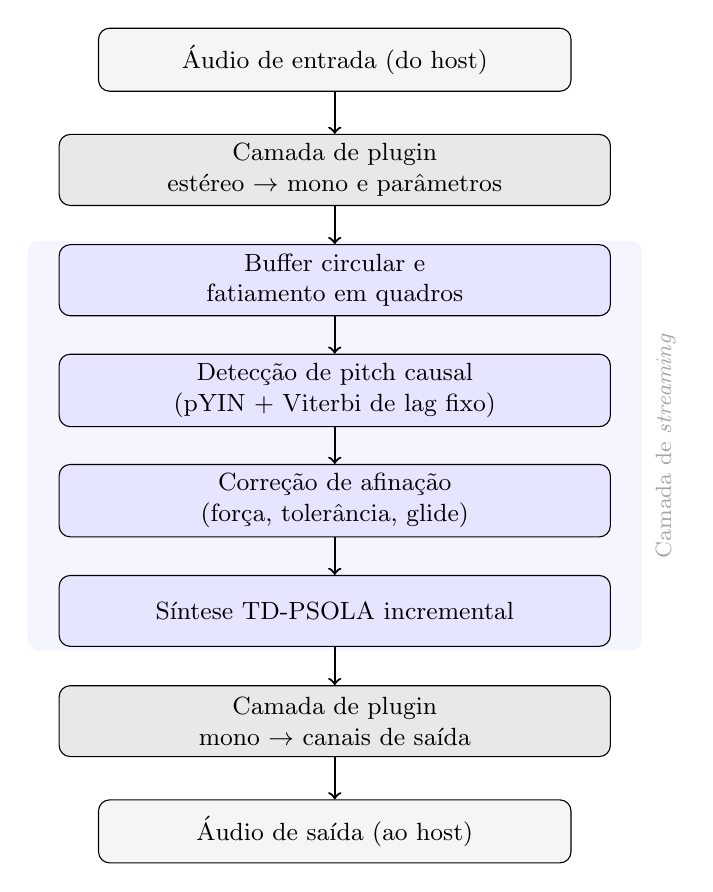
\begin{tikzpicture}[
  font=\small,
  io/.style={draw, rounded corners, minimum width=6cm, minimum height=0.8cm, align=center, fill=gray!8},
  pbox/.style={draw, rounded corners, minimum width=7cm, minimum height=0.9cm, align=center, fill=gray!18},
  sbox/.style={draw, rounded corners, minimum width=7cm, minimum height=0.9cm, align=center, fill=blue!10},
  arr/.style={->, thick}
]
  % fundo do grupo de streaming
  \fill[blue!4, rounded corners] (-3.9,-2.3) rectangle (3.9,-7.5);
  \node[rotate=90, gray!70] at (4.2,-4.9) {\footnotesize Camada de \textit{streaming}};
  % nós
  \node[io]   (n0) at (0,0)    {Áudio de entrada (do host)};
  \node[pbox] (n1) at (0,-1.4) {Camada de plugin\\ estéreo $\to$ mono e parâmetros};
  \node[sbox] (n2) at (0,-2.8) {Buffer circular e\\ fatiamento em quadros};
  \node[sbox] (n3) at (0,-4.2) {Detecção de pitch causal\\ (pYIN + Viterbi de lag fixo)};
  \node[sbox] (n4) at (0,-5.6) {Correção de afinação\\ (força, tolerância, glide)};
  \node[sbox] (n5) at (0,-7.0) {Síntese TD-PSOLA incremental};
  \node[pbox] (n6) at (0,-8.4) {Camada de plugin\\ mono $\to$ canais de saída};
  \node[io]   (n7) at (0,-9.8) {Áudio de saída (ao host)};
  % setas
  \draw[arr] (n0)--(n1);
  \draw[arr] (n1)--(n2);
  \draw[arr] (n2)--(n3);
  \draw[arr] (n3)--(n4);
  \draw[arr] (n4)--(n5);
  \draw[arr] (n5)--(n6);
  \draw[arr] (n6)--(n7);
\end{tikzpicture}
\caption{\label{fig:arquitetura}Arquitetura e fluxo de sinal do protótipo. O áudio entra pela camada de plugin (JUCE), é convertido para mono e processado pela camada de \textit{streaming} em quatro passos --- fatiamento, detecção de pitch, correção e síntese ---, retornando à camada de plugin para distribuição aos canais de saída.}
\small Fonte: Elaborada pelo autor.
\end{figure}

Além do caminho de \textit{streaming} integrado ao plugin, o protótipo inclui uma versão para linha de comando que processa um arquivo de áudio inteiro de forma causal e reporta a latência algorítmica e o fator de tempo real. Como usa a mesma matemática de detecção e síntese e sua saída é diretamente comparável ao processamento em lote, ela serviu de referência durante o desenvolvimento: qualquer divergência entre as duas versões indicava um bug no motor de \textit{streaming}. Manter essa matemática separada do motor também ajudou no diagnóstico --- diante de um comportamento inesperado, era possível isolar primeiro se o problema estava nas funções matemáticas ou na lógica de janelamento e acumulação ---, o que reduziu o tempo de depuração ao longo do trabalho.

\section{Funções de processamento de sinal}
\label{sec:impl_dsp}

\subsection{Estimação de pitch}

Detectar a afinação de uma voz é, em essência, descobrir de quanto em quanto tempo sua forma de onda se repete: esse intervalo é o período, e seu inverso é a frequência fundamental. O algoritmo pYIN mede essa repetição comparando o sinal com cópias deslocadas de si mesmo --- quando o deslocamento coincide com o período, a cópia volta a casar com o original, como ilustra a Figura~\ref{fig:autossimilaridade}.

\begin{figure}[H]
\centering
% --- (a) deslocamento que NÃO bate com o período ---
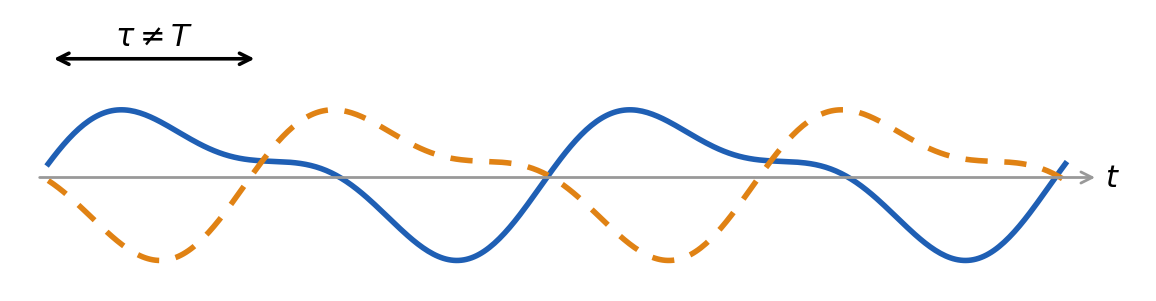
\includegraphics[width=0.82\textwidth]{fig/autossim-a.png}\\[2pt]
{\small (a) Deslocamento $\tau \neq T$: a cópia (laranja, tracejada) fica fora de fase com o original (azul). A diferença entre os dois é grande.}\\[10pt]
% --- (b) deslocamento IGUAL ao período ---
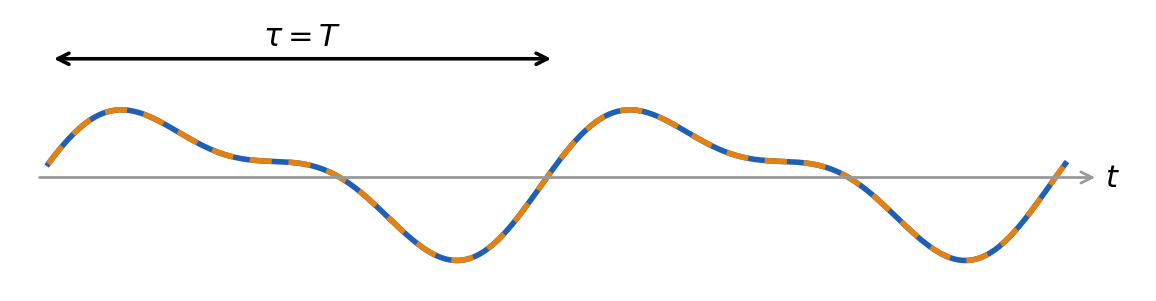
\includegraphics[width=0.82\textwidth]{fig/autossim-b.png}\\[2pt]
{\small (b) Deslocamento $\tau = T$ (um período): a cópia recai exatamente sobre o original. A diferença entre os dois cai a quase zero --- é esse mínimo que o algoritmo procura.}
\caption{\label{fig:autossimilaridade}Princípio da detecção de pitch por auto-similaridade. Comparando o sinal com uma cópia de si mesmo deslocada de $\tau$ amostras, o deslocamento que minimiza a diferença revela o período fundamental $T$.}
\small Fonte: Elaborada pelo autor.
\end{figure}

A estimação da frequência fundamental é baseada no algoritmo pYIN, que opera sobre quadros curtos do sinal de entrada \cite{mauch2014pyin,decheveigne2002yin}. Para cada quadro de $N_{\text{frame}}$ amostras, calcula-se, sobre uma janela de análise de $W = N_{\text{frame}}/2$ amostras, a função de diferença cumulativa normalizada (CMNDF), que quantifica a dissimilaridade entre o sinal e uma versão deslocada de si mesmo em $\tau$ amostras e suprime mínimos espúrios em atrasos pequenos, tornando mais saliente o mínimo correspondente ao período fundamental \cite{decheveigne2002yin}. O pYIN estende o YIN ao substituir o limiar absoluto de decisão por uma distribuição sobre $K = 100$ limiares distintos, gerando múltiplos candidatos de pitch por quadro com probabilidades associadas. Para cada limiar $s_k$, o período candidato é estimado pelo primeiro mínimo local da CMNDF abaixo de $s_k$, refinado por interpolação parabólica, e ponderado por uma distribuição Beta adaptada que favorece valores intermediários \cite{mauch2014pyin}. As expressões da CMNDF e do peso dos candidatos estão no Apêndice~\ref{ap:formulas} (Seção~\ref{ap:cmndf}).

Os candidatos gerados são acumulados em um histograma cujos bins correspondem a intervalos de $\Delta = 20$ cents entre $F_{\min}$ e $F_{\max}$, servindo de observação para o modelo oculto de Markov descrito na Seção~\ref{sec:impl_streaming}. Os parâmetros adotados foram $N_{\text{frame}} = 1024$ amostras e $N_{\text{hop}} = 256$ amostras, consistentes com a configuração escolhida no Capítulo~\ref{chap:resultados}.

\subsection{Correção de afinação}

Conhecida a frequência cantada, corrigir a afinação se resume a três decisões: descobrir qual nota o cantor pretendia atingir, medir o quanto ele se desviou dela e empurrar o som de volta à nota certa --- preservando pequenos desvios intencionais e permitindo dosar a intensidade da correção.

A partir da frequência fundamental estimada $f$, a nota-alvo é determinada convertendo $f$ em nota MIDI contínua ($m = 69 + 12\log_2(f/440)$) e identificando a nota inteira mais próxima pertencente à escala configurada, denominada $m^*$. O erro de afinação em cents é $e = (m^* - m) \cdot 100$. Uma tolerância --- também chamada de \textit{zona morta} --- de largura $\delta$ preserva pequenos desvios intencionais, como vibrato e microafinação: se $|e| \leq \delta$, nenhuma correção é aplicada. Caso contrário, o deslocamento residual é amplificado pelo parâmetro de força $\gamma \in [0,1]$:

\begin{equation}
f_{\text{out}} = 440 \cdot 2^{\;\bigl(m \;+\; \gamma \cdot \operatorname{sgn}(e) \cdot (|e| - \delta)\;/\;100\bigr)\;/\;12 \;-\; 69/12}
\end{equation}

Em termos práticos, a equação apenas reconstrói a frequência de saída a partir da nota já corrigida. Com $\gamma = 0$, tem-se $f_{\text{out}} = f$ e o sinal passa intacto; com $\gamma = 1$, o desvio que excede a tolerância é integralmente removido, levando a voz à nota-alvo (a menos da própria largura $\delta$ da tolerância); valores intermediários aplicam uma fração proporcional da correção, permitindo desde um ajuste sutil até o efeito de afinação duro.

A escala de referência é configurável entre cromática e as principais tonalidades maiores e menores, determinando quais classes de nota são elegíveis como alvo. A faixa de busca de pitch $[F_{\min}, F_{\max}]$ é selecionada por presets de tessitura vocal alinhados à classificação SATB \cite{aalto_speech_properties}, apresentados na Tabela~\ref{tab:presets_tessitura}. Essa faixa influencia tanto a qualidade da detecção quanto a latência do sistema, uma vez que a folga de guarda da síntese cresce com $f_s / F_{\min}$: tessituras mais graves exigem folga maior e, portanto, resultam em latência total mais elevada.

A escolha do preset não é arbitrária. Para verificá-la empiricamente, uma gravação real de uma cantora contralto --- cujo grave cantado fica em torno de Sol$_3$ (193~Hz) e cuja mediana de pitch é próxima de Lá$\sharp_3$ (230~Hz) --- foi processada com os seis presets vocais. O preset de contralto ($F_{\min} = 175$~Hz) não perdeu nenhuma nota (0\% de notas abaixo da faixa de busca) e obteve a melhor similaridade com a referência offline (0{,}236)\footnote{Ao longo do texto, a \emph{similaridade} entre uma saída causal e a saída de referência --- o processamento em lote do mesmo algoritmo, tomado como ``ouro'' --- é medida como a média, sobre janelas de $0{,}5$~s, do coeficiente de correlação de Pearson entre as duas formas de onda, descartando as janelas silenciosas; o valor $1{,}0$ indica saídas idênticas. Por comparar diretamente as formas de onda ressintetizadas por TD-PSOLA, sensíveis a pequenas diferenças de fase, os valores absolutos são baixos, mas preservam a ordenação relativa entre as configurações comparadas.}; por ter o maior $F_{\min}$ entre os presets que preservam toda a voz, é também o de menor latência entre eles. Os presets mais graves --- baixo, barítono e tenor --- também não perderam notas, mas resultaram em latência maior e qualidade pior, pois sua grade de busca de pitch é mais ampla que o necessário e induz mais erros de oitava no Viterbi causal. No sentido oposto, o preset de mezzo ($F_{\min} = 220$~Hz) perdeu 25{,}9\% das notas, que caem abaixo de $F_{\min}$ e permanecem sem correção, e o de soprano ($F_{\min} = 262$~Hz) perdeu 98{,}4\%. O padrão é claro: o preset ideal é o de maior $F_{\min}$ que ainda não perde nenhuma nota da voz real, pois isso minimiza a latência e maximiza a qualidade ao mesmo tempo --- não há, nesse ponto, um compromisso entre as duas grandezas.

\begin{table}[H]
\centering
\caption{\label{tab:presets_tessitura}Presets de tessitura e faixas de busca de pitch correspondentes.}
\small
\begin{tabular}{|p{3.0cm}|p{2.5cm}|p{2.5cm}|p{6.0cm}|}
\hline
\textbf{Preset} & \textbf{$F_{\min}$ (Hz)} & \textbf{$F_{\max}$ (Hz)} & \textbf{Faixa aproximada} \\
\hline
Baixo       & 82  & 330  & Mi$_2$ -- Mi$_4$ \\
\hline
Barítono    & 98  & 392  & Sol$_2$ -- Sol$_4$ \\
\hline
Tenor       & 131 & 523  & Dó$_3$ -- Dó$_5$ \\
\hline
Contralto   & 175 & 698  & Fá$_3$ -- Fá$_5$ \\
\hline
Mezzo       & 220 & 880  & Lá$_3$ -- Lá$_5$ \\
\hline
Soprano     & 262 & 1047 & Dó$_4$ -- Dó$_6$ \\
\hline
Instrumento & 50  & 2000 & Faixa ampla \\
\hline
\end{tabular}
\small Fonte: Elaborada pelo autor.
\end{table}

\subsection{Síntese TD-PSOLA}

Mudar a altura de um som sem alterar sua duração é o cerne da correção de afinação. O TD-PSOLA faz isso recortando o trecho vocal em pequenos grãos, cada um com cerca de dois períodos de largura, e reposicionando-os com um espaçamento diferente: mais apertado para subir a afinação, mais largo para baixá-la. Como cada grão preserva a forma local da onda --- e, portanto, o timbre da voz --- e os grãos são redistribuídos ao longo da mesma janela de tempo, a altura muda sem que a duração ou o caráter da voz se alterem, como ilustra a Figura~\ref{fig:psola_graos}.

\begin{figure}[H]
\centering
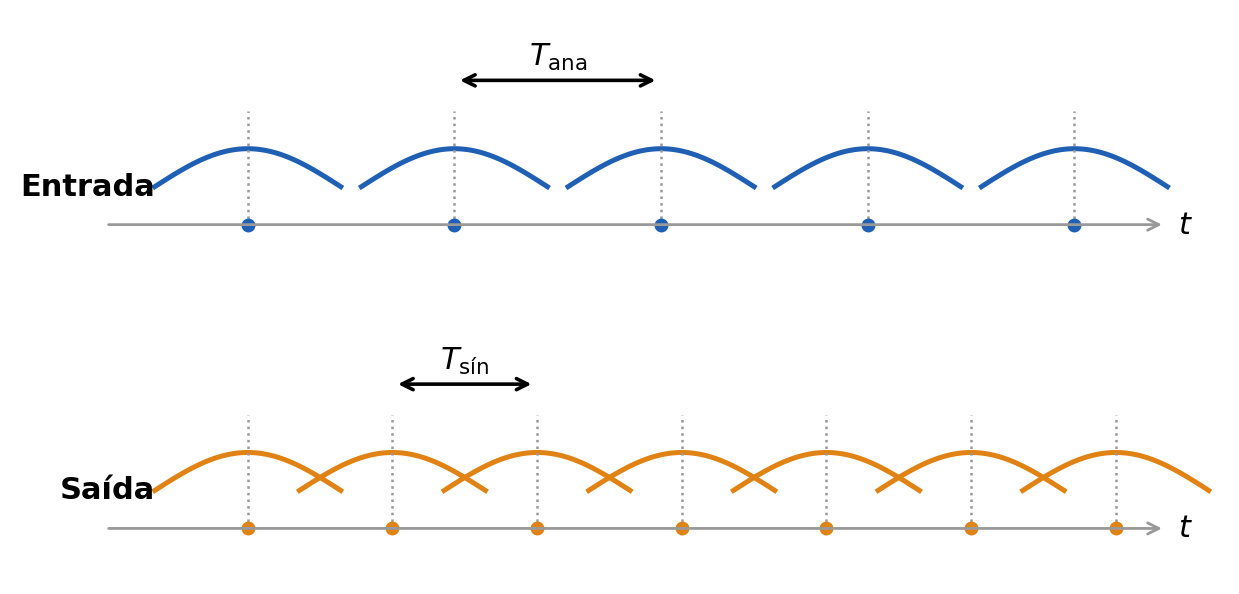
\includegraphics[width=0.85\textwidth]{fig/psola-graos.png}
\caption{\label{fig:psola_graos}Princípio do TD-PSOLA para elevação de afinação. O sinal de entrada é decomposto em grãos (janelas de Hann) centrados nas marcas de análise, espaçadas de um período $T_{\text{ana}}$. Para subir a afinação, os grãos são reposicionados com espaçamento menor $T_{\text{sín}} < T_{\text{ana}}$; como ocupam a mesma janela de tempo (à custa de um número maior de grãos), a duração do trecho é preservada.}
\small Fonte: Elaborada pelo autor.
\end{figure}

A correção de pitch é realizada pela técnica TD-PSOLA (\textit{Time-Domain Pitch-Synchronous Overlap-Add}) \cite{moulines1990psola,aalto_psola}. O algoritmo recebe o sinal de entrada, a trajetória de $F_0$ real por amostra e a trajetória de pitch-alvo por amostra, e produz o sinal corrigido em três etapas.

Na primeira, são determinadas as marcas de análise, posicionadas uma por período ao longo das regiões vozeadas do sinal. A primeira marca de cada região ancora-se no pico de maior amplitude; as marcas seguintes são posicionadas por correlação cruzada com o entorno da marca anterior, garantindo coerência de fase entre grãos consecutivos.

Na segunda, os grãos de síntese são posicionados nas marcas de análise reamostradas de acordo com a razão de transposição local $\beta = F_{\text{out}} / F_0$, sobrepostos por uma janela de Hann de meia-largura $L = T_{\text{ana}}$. A preservação de duração é garantida pelo fato de que as posições de síntese são determinadas localmente, sem dependência do comprimento total da região vozeada, o que torna o algoritmo adequado para uso em janela deslizante no contexto de \textit{streaming}. As expressões do posicionamento das marcas (por correlação cruzada) e da sobreposição dos grãos estão no Apêndice~\ref{ap:formulas} (Seção~\ref{ap:psola}).

Na terceira, as regiões sem marcas de análise --- trechos não vozeados, transientes ou o início do sinal --- são preenchidas pelo sinal original sem processamento, combinado ao sinal sintetizado por uma rampa gradual, evitando descontinuidades audíveis nas transições.

\section{Núcleo de processamento em tempo real}
\label{sec:impl_streaming}

O motor de \textit{streaming} encapsula o autotune em um formato compatível com o protocolo de plugins de áudio: o host configura o motor uma vez, com taxa de amostragem e parâmetros, e em seguida o alimenta repetidamente com blocos de tamanho arbitrário. O motor foi desenvolvido em etapas incrementais, partindo de um passthrough simples e acrescentando cada componente sobre o anterior, de modo que qualquer divergência em relação à versão de referência pudesse ser identificada e isolada assim que surgisse.

A cada bloco de áudio recebido, o motor executa quatro passos em sequência: (1)~acumula as amostras e as fatia em quadros de análise de tamanho fixo; (2)~estima o pitch de cada quadro de forma causal, com look-ahead limitado; (3)~converte o pitch detectado em pitch-alvo, aplicando força, tolerância e glide; e (4)~sintetiza a saída corrigida de forma incremental. Cada um desses passos é detalhado a seguir, e a equivalência do resultado com o processamento offline é verificada ao final da seção.

\subsection{Buffer circular e fatiamento de quadros}

O host pode entregar o áudio em blocos de tamanho arbitrário, mas o detector de pitch só trabalha com janelas de tamanho fixo. Este componente faz a ponte entre os dois.

As amostras recebidas em cada chamada são escritas em um buffer circular de capacidade ligeiramente superior a $N_{\text{frame}}$. Isso garante que sempre exista ao menos um quadro completo disponível para análise, qualquer que seja o tamanho do bloco recebido. Um novo quadro de análise é disparado quando duas condições se cumprem ao mesmo tempo: há amostras acumuladas suficientes para preencher uma janela de $N_{\text{frame}}$ amostras, e pelo menos $N_{\text{hop}}$ amostras chegaram desde o último quadro. Se o bloco do host for maior que $N_{\text{hop}}$, vários quadros podem ser disparados numa única chamada. Em todos os casos, a sequência de quadros produzida é independente do tamanho de bloco e reproduz exatamente o fatiamento que seria obtido sobre o sinal inteiro.

\subsection{Detecção de pitch causal com Viterbi de lag fixo}

Na versão offline, o Viterbi enxerga a trajetória de pitch inteira antes de decidir cada nota: pode ``olhar o futuro'' para corrigir uma decisão passada. Ao vivo isso é impossível, pois a estimativa de cada quadro precisa ser emitida com atraso mínimo, sem esperar o restante da música. A solução adotada é deixar o algoritmo espiar apenas alguns quadros à frente --- o \textit{look-ahead} --- antes de comprometer definitivamente cada decisão, equilibrando qualidade e latência.

A análise de pitch é executada sobre cada quadro fatiado, replicando de forma causal e incremental a matemática da versão de referência. O processo compreende duas operações por quadro.

A primeira calcula a observação do quadro: a CMNDF é computada sobre as $W = N_{\text{frame}}/2$ amostras do quadro, os $K = 100$ candidatos de pitch com os respectivos pesos pYIN são gerados e acumulados em um histograma de bins de pitch \cite{mauch2014pyin}. A massa total acumulada corresponde à probabilidade de vozeamento do quadro; o complemento representa a probabilidade de ausência de voz.

A segunda executa um passo do algoritmo de Viterbi sobre o modelo oculto de Markov descrito na Seção~\ref{sec:impl_dsp}. O modelo possui um estado para cada bin de pitch e um estado adicional para trechos não vozeados, com probabilidades de transição que penalizam saltos de pitch grandes e favorecem a continuidade temporal da trajetória. A cada quadro, a pontuação de cada altura possível combina duas evidências: o quão bem ela explica o som efetivamente ouvido e o quanto dá continuidade à melhor trajetória vinda do quadro anterior. A recursão de Viterbi correspondente está no Apêndice~\ref{ap:formulas} (Seção~\ref{ap:viterbi}).

Em vez de armazenar todas as colunas de retrocesso --- o que exigiria memória crescente com o tempo --- o motor mantém apenas as últimas $L + 1$ colunas, onde $L$ é o parâmetro de lag configurável. Assim que esse número de colunas se acumula, a estimativa de $F_0$ do quadro mais antigo é emitida retrotraçando $L$ passos: parte-se do melhor estado da coluna atual e segue-se a cadeia de ponteiros de retrocesso para trás, um quadro de cada vez, até alcançar o quadro de $L$ passos atrás --- cuja estimativa de $F_0$, já amadurecida pelo contexto dos quadros seguintes, é então emitida (expressão no Apêndice~\ref{ap:formulas}, Seção~\ref{ap:viterbi}).

Esse mecanismo de lag fixo é equivalente ao Viterbi global \cite{mauch2014pyin} quando $L \to \infty$, aproximando-se progressivamente da qualidade do processamento offline à medida que o lag aumenta, ao custo de uma latência adicional de $L \cdot N_{\text{hop}}$ amostras.

\subsection{Emissão de amostras e filtro de glide}

Com o pitch disponível, o motor preenche, para cada quadro emitido, $N_{\text{hop}}$ posições de dois vetores paralelos: um com o pitch real detectado por amostra e outro com o pitch-alvo por amostra, já com os efeitos de força, tolerância e glide aplicados.

O filtro de glide modela o deslizamento gradual da correção em direção à nota-alvo, suavizando transições abruptas que, sem ele, soariam artificiais e robóticas --- o som mecânico típico de autotune exagerado. Operando em escala logarítmica de cents, o filtro é definido como um filtro de primeira ordem:

\begin{equation}
\label{eq:glide}
g[n] = \alpha \cdot g[n-1] + (1-\alpha) \cdot c_{\text{alvo}}[n], \quad \alpha = e^{-1/(\tau \cdot f_s)}
\end{equation}

onde $\tau$ é o tempo de glide em segundos e $c_{\text{alvo}}[n]$ é o pitch-alvo expresso em cents. O estado do filtro é reiniciado no início de cada região vozeada, de modo que a primeira nota de uma frase vocal seja atingida de forma direta, sem arraste do período de silêncio anterior. A saída em Hz é recuperada pela inversa da conversão logarítmica.

O efeito dos valores mais altos de glide só ficou evidente durante os testes do plugin no Ableton Live \cite{ableton_live}: ao levar o tempo de glide ao máximo, a correção passou a soar estranha e desafinada em algumas frases, e foi acompanhando esse comportamento se entendeu o que o parâmetro controla. Valores baixos produzem o ``snap'' característico do autotune, em que a nota atinge a afinação alvo quase instantaneamente. Valores altos suavizam as transições, mas, levados ao extremo, expõem um efeito colateral que só apareceu ao monitorar transições rápidas: numa troca veloz entre notas, o alvo glidado ainda está deslizando, saindo da nota anterior, enquanto o cantor já entoa a seguinte. O sintetizador então puxa um trecho que já estava correto para um pitch intermediário, que não corresponde a nenhuma nota da escala, e o resultado soa desafinado --- pior, inclusive, que o sinal sem correção. Foi esse teste que deixou claro que o regime extremo descaracteriza o autotune.

\subsection{Síntese TD-PSOLA incremental}

A geração da saída corrigida é feita de forma incremental, sem modificar o algoritmo de síntese descrito na Seção~\ref{sec:impl_dsp}. A estratégia adotada foi a de janela deslizante com \textit{overlap-save}: a cada chamada, o algoritmo de síntese é reaplicado sobre uma janela do sinal acumulado que se estende de uma margem anterior à fronteira já finalizada até a fronteira de decisão atual. Apenas o segmento novo --- as amostras que ainda não haviam sido comprometidas na chamada anterior --- é então registrado no buffer de saída.

A fronteira de decisão é definida como o número de amostras para as quais o pitch-alvo já foi emitido, descontada uma folga de guarda $p_{\text{guard}}$ de dois períodos do tom mais grave configurado --- ou seja, proporcional a $f_s / F_{\min}$ (expressão no Apêndice~\ref{ap:formulas}, Seção~\ref{ap:guarda}). Essa folga garante que o último grão de síntese de cada janela nunca alcance a região ainda não finalizada, produzindo uma saída numericamente idêntica à que seria obtida pelo processamento do sinal inteiro em lote.

Durante os testes da síntese incremental, surgiram estalos audíveis nos casos em que uma nota sustentada era entregue ao motor em vários blocos sucessivos, ainda em andamento. O diagnóstico comparou a saída do motor de \textit{streaming}, amostra a amostra, com a da versão em lote: as divergências apareciam justamente quando uma nova janela deslizante começava no meio de uma região vozeada já parcialmente sintetizada em chamadas anteriores. A causa era a posição da âncora: o algoritmo de TD-PSOLA localiza a primeira marca de análise de cada região vozeada pelo pico de maior amplitude dentro dela; se a janela deslizante começasse no meio da região, ela enxergava esse trecho como uma região ``nova'' e escolhia um pico diferente do que a versão em lote teria escolhido para a mesma região, produzindo uma sequência de grãos com fase inconsistente em relação ao que já havia sido sintetizado --- o que se ouvia como um estampido na junção entre uma janela e a próxima. A correção foi recuar o início de cada janela deslizante até o início real da região vozeada corrente, garantindo que toda janela que cubra aquela região compartilhe sempre a mesma âncora --- e, portanto, a mesma sequência de grãos --- que a versão em lote produziria.

A latência algorítmica total reportada ao host, que permite ao Ableton Live \cite{ableton_live} compensar o atraso e manter o sincronismo com as demais faixas do projeto, é:

\begin{equation}
\label{eq:latencia_total}
L_{\text{total}} = N_{\text{frame}} + L \cdot N_{\text{hop}} + p_{\text{guard}}
\end{equation}

onde o primeiro termo corresponde ao quadro de análise de pitch, o segundo ao lag do Viterbi e o terceiro à folga de síntese. Com os parâmetros padrão ($N_{\text{frame}} = 1024$, $L = 4$, $N_{\text{hop}} = 256$, $F_{\min} = 175$~Hz para a tessitura de contralto, $f_s = 44{.}100$~Hz), a latência total é de aproximadamente 58~ms. Para tessituras mais agudas, em que $F_{\min}$ é maior, $p_{\text{guard}}$ diminui e a latência total se reduz proporcionalmente.

Convém distinguir essa latência total da cadeia de correção da latência de detecção de pitch usada como critério no estudo comparativo (Capítulo~\ref{chap:resultados}): aquela varredura considerou apenas o quadro de análise (cerca de 23~ms para $N_{\text{frame}} = 1024$), enquanto a cadeia causal completa soma ainda o lag do Viterbi e a folga de síntese do TD-PSOLA, totalizando os $\approx 58$~ms acima. Esse valor situa-se acima do teto de 20--30~ms desejável para monitoração ao vivo estrita; trata-se, porém, de uma latência estrutural e parametrizável (reduz-se com \textit{look-ahead} menor ou tessituras mais agudas) e reportada ao host para compensação de atraso, o que permite o alinhamento com as demais faixas em contexto de mixagem.

A escolha do valor padrão de look-ahead resulta de uma varredura desse parâmetro no motor causal de referência, que implementa a mesma lógica de Viterbi de lag fixo e não está sujeito ao limite de faixa exposto na interface do plugin, o que permite estender a varredura além do máximo oferecido ao usuário. A Tabela~\ref{tab:sweep_lookahead} apresenta o compromisso entre latência e qualidade em função do número de quadros de look-ahead; os valores absolutos de latência diferem do exemplo anterior por terem sido medidos nessa configuração de referência, mas o formato da curva é o que importa para justificar a escolha do parâmetro.

\begin{table}[H]
\centering
\caption{\label{tab:sweep_lookahead}Compromisso entre latência e qualidade em função do look-ahead.}
\small
\begin{tabular}{|p{3.5cm}|p{3.0cm}|p{5.5cm}|}
\hline
\textbf{Look-ahead (quadros)} & \textbf{Latência} & \textbf{Similaridade com a saída offline} \\
\hline
0  & 41{,}5~ms & 0{,}562 \\
\hline
2  & 53{,}1~ms & 0{,}560 \\
\hline
4  & 64{,}7~ms & 0{,}654 \\
\hline
8  & 88{,}0~ms & 0{,}740 \\
\hline
16 & 134~ms    & 0{,}740 \\
\hline
32 & 227~ms    & 0{,}740 \\
\hline
\end{tabular}
\small Fonte: Elaborada pelo autor.
\end{table}

A qualidade cresce com o look-ahead até cerca de oito quadros, ponto em que satura em torno de 0{,}740; acima disso, o aumento do parâmetro apenas acrescenta latência sem ganho de qualidade. O custo computacional não é o fator limitante: no caminho \textit{offline} de referência, o fator de tempo real medido permaneceu constante em aproximadamente 0{,}025 --- cerca de 40 vezes mais rápido que o tempo real --- em todos os valores de look-ahead testados, o que confirma que a latência é uma escolha estrutural do algoritmo, e não uma restrição imposta pela CPU. Cabe registrar que essa medição corresponde ao processamento em lote de referência; o custo por bloco do motor de \textit{streaming} integrado ao plugin não foi caracterizado de forma sistemática nesta etapa, ficando como item da avaliação de desempenho prevista para a continuidade do trabalho. O valor padrão adotado no plugin (look-ahead de 4 quadros) situa-se deliberadamente antes do ponto de saturação: privilegia a baixa latência exigida pela monitoração ao vivo, aceitando uma qualidade um pouco abaixo do ótimo (0{,}654 contra 0{,}740) em troca de uma latência sensivelmente menor (64{,}7~ms contra 88{,}0~ms).

\subsection{Verificação}

A equivalência entre o motor de \textit{streaming} e a versão em lote, adotada como referência (\textit{gold}), foi avaliada por um conjunto de testes automatizados. O fatiamento do sinal em quadros de análise é idêntico ao da versão em lote para blocos de 64, 128, 256 e 512 amostras, confirmando que a sequência de quadros independe do tamanho de bloco entregue pelo host. A trilha de frequência fundamental estimada pelo motor causal coincide com a da versão em lote em mais de 99\% dos quadros vozeados --- descontados os primeiros quadros, ainda sob influência do \textit{look-ahead} --- e a saída final corrigida apresenta correlação de 0{,}997 com a referência \textit{offline}; o resíduo é atribuído a um jitter de fase inferior a três amostras por nota. Com a força de correção em zero, a saída reproduz a entrada sem alteração audível.

\section{Integração com JUCE}
\label{sec:impl_juce}

\subsection{Parâmetros expostos ao host}

A integração com o framework JUCE \cite{juce_website,juce_github} segue a arquitetura padrão de plugins de áudio: o processador declara um conjunto de parâmetros que são expostos ao host, salvos junto ao projeto e sincronizados automaticamente com a interface gráfica. O protótipo expõe seis parâmetros, divididos em dois grupos conforme seu impacto sobre o motor, descritos na Tabela~\ref{tab:parametros_plugin}.

\begin{table}[H]
\centering
\caption{\label{tab:parametros_plugin}Parâmetros do plugin expostos ao host.}
\small
\begin{tabular}{|p{2.8cm}|p{2.8cm}|p{2.4cm}|p{5.5cm}|}
\hline
\textbf{Parâmetro} & \textbf{Tipo / Faixa} & \textbf{Padrão} & \textbf{Descrição} \\
\hline
Força          & Float $[0, 1]$         & 1{,}0      & Intensidade da correção: 0 = sem correção; 1 = correção máxima. \\
\hline
Tolerância     & Float $[0, 50]$ cents  & 15 cents   & Desvios menores que este valor não são corrigidos, preservando vibrato e microafinação. \\
\hline
Glide          & Float $[0, 200]$ ms    & 40 ms      & Tempo de deslizamento até a nota-alvo; reduz o efeito de correção abrupta. \\
\hline
Look-ahead     & Inteiro $[0, 16]$      & 4 quadros  & Lag do Viterbi: maior valor melhora a qualidade da detecção ao custo de maior latência. \textit{Estrutural.} \\
\hline
Voz            & Seleção (7 opções)     & Contralto  & Preset de tessitura: define $F_{\min}$ e $F_{\max}$ da busca de pitch. \textit{Estrutural.} \\
\hline
Escala         & Seleção (7 opções)     & Cromática  & Escala de referência para a correção. \textit{Estrutural.} \\
\hline
\end{tabular}
\small Fonte: Elaborada pelo autor.
\end{table}

Os parâmetros marcados como \textit{estruturais} --- look-ahead, voz e escala --- modificam o espaço de estados do modelo oculto de Markov do pYIN (Seção~\ref{sec:impl_streaming}), a profundidade temporal do algoritmo de Viterbi ou a faixa de busca de pitch, exigindo reconfiguração completa quando alterados. Quando tal alteração é detectada, o motor é reconfigurado antes de processar o bloco corrente, e a nova latência algorítmica é comunicada ao host para atualização da compensação de atraso. Os demais parâmetros --- força, tolerância e glide --- podem ser ajustados continuamente durante a execução sem qualquer reconfiguração ou realocação de memória.

\subsection{Processamento bloco a bloco}

A cada bloco de áudio, o processador verifica se algum parâmetro estrutural foi alterado e, em caso positivo, reconfigura o motor antes de prosseguir. Em seguida, os parâmetros de ajuste contínuo são atualizados no motor e o sinal de entrada --- que pode ser estéreo --- é convertido para mono por média dos canais, processado pelo motor de \textit{streaming} e distribuído de volta para todos os canais de saída.

O protótipo foi carregado e executado em tempo real no Ableton Live \cite{ableton_live}, processando voz ao vivo sem falhas perceptíveis nos testes realizados (Figura~\ref{fig:autotune_gui}). Ainda assim, o núcleo de processamento desta versão (MVP) realiza alocações de memória no caminho de áudio a cada bloco, herdadas da implementação \textit{offline} reaproveitada: na prática elas cabem no prazo de processamento do bloco, mas não constituem garantia formal de operação livre de falhas sob sessões longas ou condições adversas. A eliminação dessas alocações --- por meio de \textit{buffers} de tamanho fixo pré-alocados, requisito para um plugin robusto em processamento em tempo real --- está prevista para a etapa seguinte do trabalho (Capítulo~\ref{chap:cronograma}). A reconfiguração estrutural, por envolver realocação, ocorre apenas quando o usuário altera explicitamente um dos parâmetros que a exigem.

\section{Interface gráfica}
\label{sec:impl_gui}

A interface gráfica do plugin é composta por duas áreas dispostas verticalmente. A área superior, que ocupa aproximadamente dois terços da janela, exibe um afinador em tempo real. A área inferior reúne os controles de parâmetros do sistema.

O afinador exibe, durante a execução, o nome da nota-alvo mais próxima da escala configurada, em destaque tipográfico; as frequências detectada e alvo em Hz; e um medidor horizontal de desvio de afinação, com faixa de $-50$ a $+50$ cents. O medidor apresenta duas marcas distintas: uma indicando o desvio da voz original em relação à nota-alvo antes da correção, e outra indicando o desvio da saída corrigida após o processamento. Essa representação visual permite avaliar, de forma imediata, o quanto a correção está deslocando o sinal vocal em direção à nota de referência. As informações são atualizadas aproximadamente 30 vezes por segundo, de forma independente do processamento de áudio.

A faixa de controles inferior reúne os seis parâmetros descritos na Tabela~\ref{tab:parametros_plugin}: os seletores de voz e escala e os quatro controles deslizantes de força, tolerância, glide e look-ahead. Qualquer alteração nesses controles é automaticamente propagada ao motor de processamento e salva no projeto do host.

A Figura~\ref{fig:autotune_gui} apresenta duas capturas de tela do plugin em execução dentro do Ableton Live \cite{ableton_live}. Na imagem à esquerda, nenhuma voz está sendo detectada e o afinador permanece em repouso. Na imagem à direita, o plugin identificou a nota Sol$_3$ (194{,}2~Hz), determinou Sol$_3$ como nota-alvo dentro da escala cromática (196{,}0~Hz) e exibe as duas marcas no medidor, evidenciando o estado de correção em andamento.

\begin{figure}[H]
    \centering
    \begin{minipage}[t]{0.47\textwidth}
        \centering
        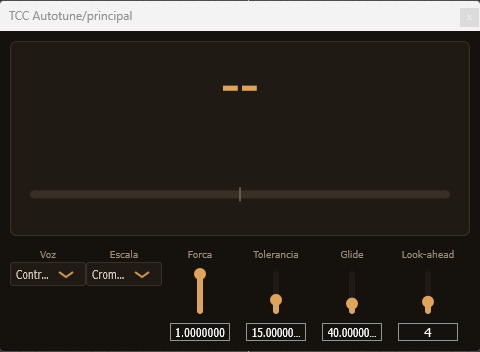
\includegraphics[width=\textwidth]{fig/autotune-plugin-repouso.png}
        \small (a) Plugin em repouso (sem voz detectada).
    \end{minipage}
    \hfill
    \begin{minipage}[t]{0.47\textwidth}
        \centering
        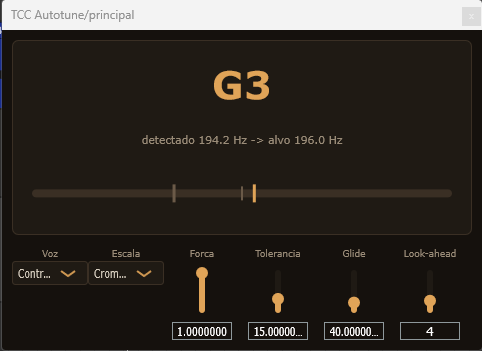
\includegraphics[width=\textwidth]{fig/autotune-plugin-funcionando.png}
        \small (b) Plugin com voz ativa: Sol$_3$ detectado (194{,}2~Hz $\to$ 196{,}0~Hz).
    \end{minipage}
    \caption{Interface gráfica do protótipo \textit{TCC Autotune} carregado no Ableton Live.}
    \label{fig:autotune_gui}
    \small Fonte: Elaborada pelo autor.
\end{figure}

\section{\label{sec:repositorio}Disponibilização do código, exemplos e materiais}

\subsection{Repositório do código}

Para permitir o acompanhamento do andamento do trabalho e a reprodução dos
resultados, o código-fonte é mantido em repositório público. O estudo comparativo
dos algoritmos de detecção de pitch, conduzido em Python (Capítulo~\ref{chap:resultados}),
está disponível em:

\begin{quote}
\url{https://github.com/gacherubini/TCC-autotune-python}
\end{quote}

O código do protótipo de autotune em C++ com JUCE (este capítulo) está disponível em:

\begin{quote}
\url{https://github.com/gacherubini/TCC-autotune-cpp}
\end{quote}

\subsection{Exemplos de áudio}
Para que o leitor possa perceber o efeito da correção, são disponibilizados,
no repositório, os arquivos de áudio antes e depois do ajuste de afinação, junto
das instruções para reprodução. A Figura~\ref{fig:exemplo_antes_depois} apresenta
a comparação visual entre o sinal original e o corrigido, por meio da trajetória
de afinação (em semitons) e do espectrograma, contrastando dois ajustes do
protótipo --- uma correção natural e uma correção forte --- e permitindo observar
o deslocamento da afinação em direção às notas-alvo.

\begin{figure}[H]
\centering
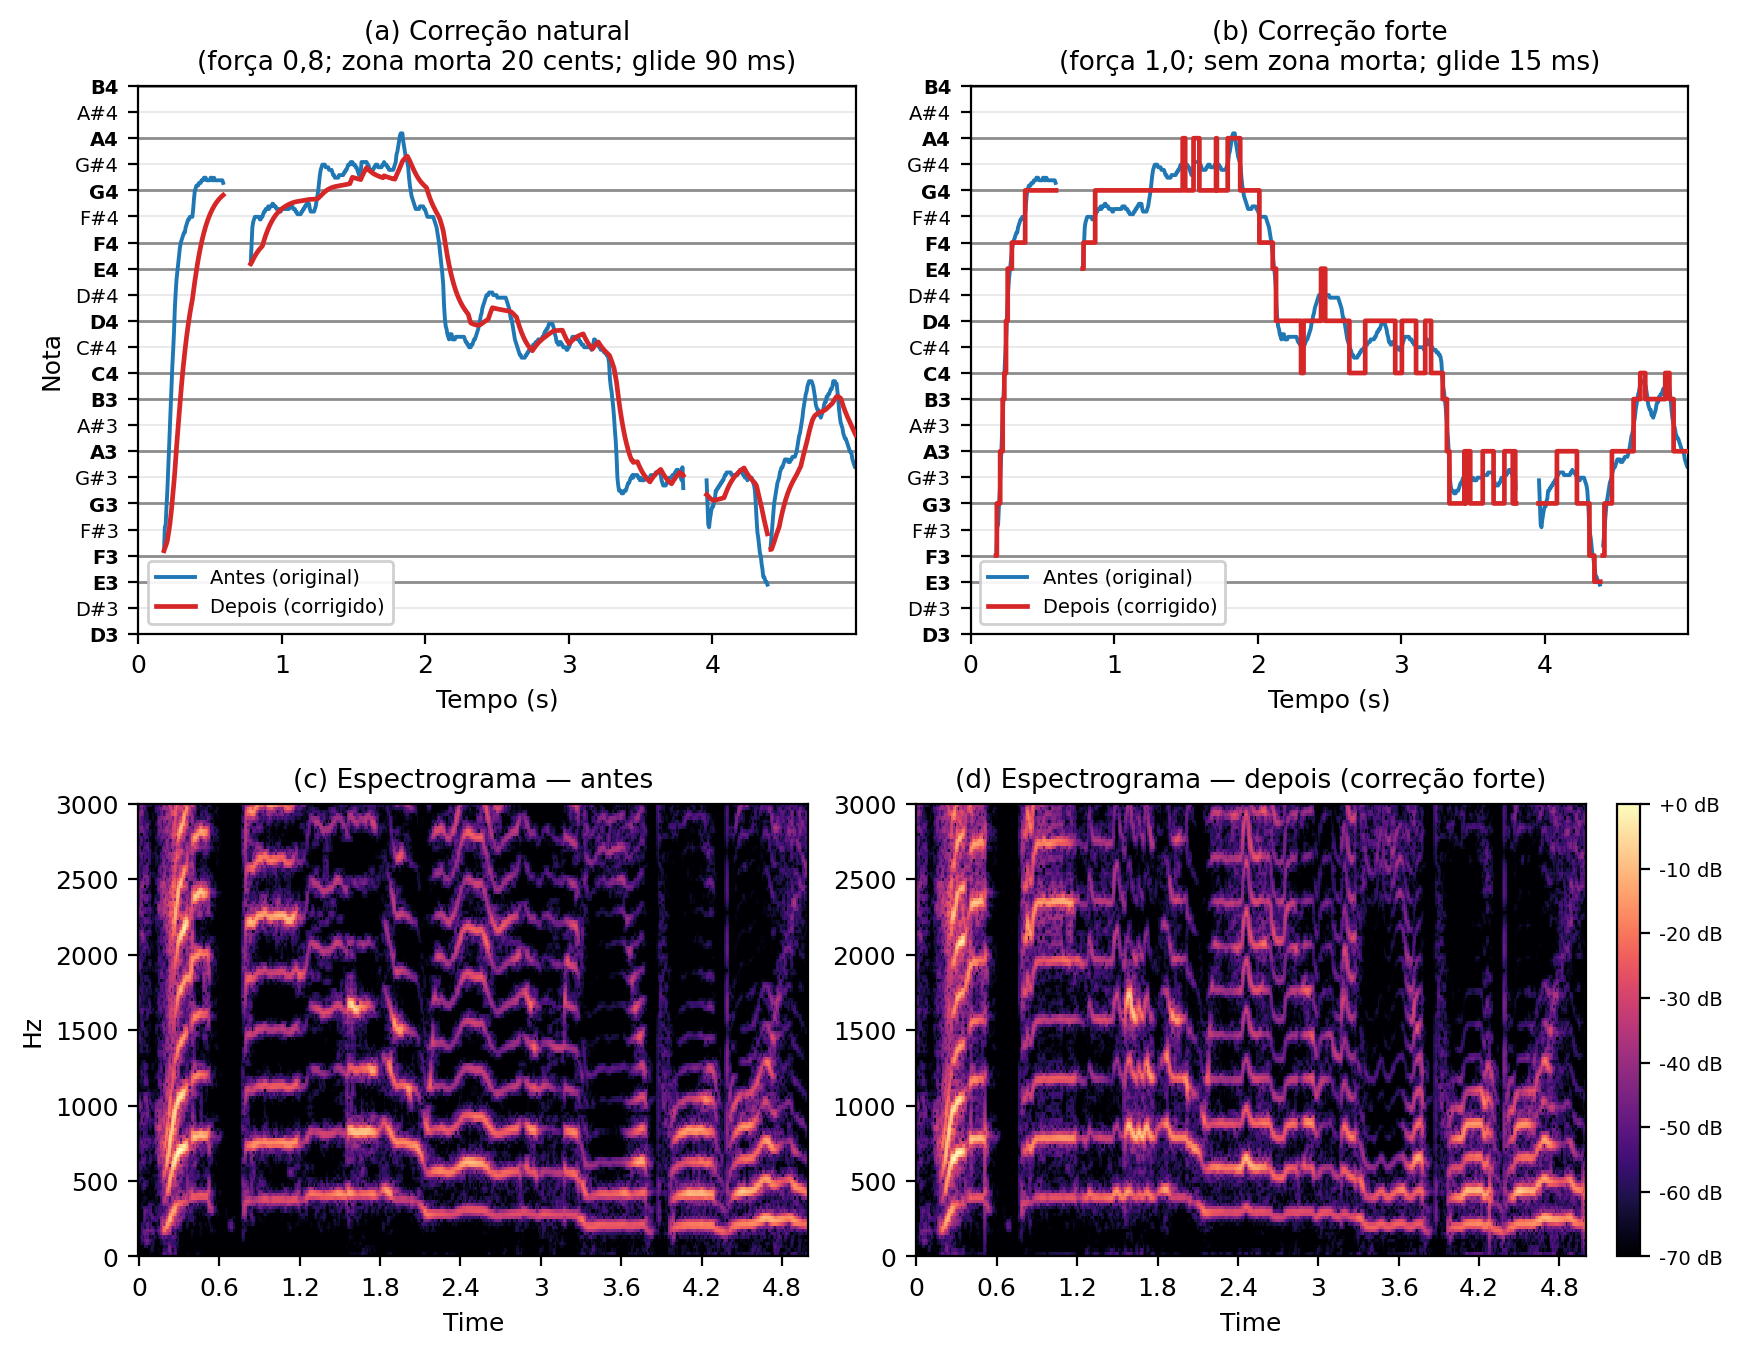
\includegraphics[width=\textwidth]{fig/exemplo-antes-depois.png}
\caption{\label{fig:exemplo_antes_depois}Comparação visual entre o áudio original
e o corrigido pelo protótipo, em um excerto de voz cantada do conjunto
\textit{Vocadito} \cite{bittner2022vocadito_zenodo}, com correção para a escala de
Dó maior (linhas e rótulos em negrito indicam as notas da escala). Os painéis (a) e
(b) contrastam dois ajustes sobre o mesmo sinal original (em azul): em (a), uma
correção natural (força parcial, tolerância de 20 cents e glide de 90~ms) acompanha
a melodia suavemente, preservando o vibrato; em (b), uma correção forte (força
total, sem tolerância e glide curto) encaixa a afinação em degraus sobre as notas
da escala. Os painéis (c) e (d) apresentam os espectrogramas antes e depois,
evidenciando a preservação da estrutura harmônica e do timbre.}
\small Fonte: Elaborada pelo autor, a partir de áudio do conjunto \textit{Vocadito} \cite{bittner2022vocadito_zenodo}.
\end{figure}

\chapter{\label{chap:conclusao}Conclusão}

Este capítulo sintetiza o estado atual do trabalho ao final desta etapa,
retomando os requisitos definidos na proposta, indicando quais foram atingidos,
registrando as principais alterações realizadas em relação ao que havia sido
planejado e apontando a continuidade prevista para a etapa seguinte.

\section{Contribuições do trabalho}

Além da entrega de um protótipo funcional, este trabalho reúne três contribuições principais. A primeira é a constatação de que, para correção automática de afinação, a \emph{estabilidade temporal} da trajetória de pitch --- e não a precisão média --- é o fator decisivo na escolha do algoritmo, uma vez que o deslocamento de pitch amplifica oscilações entre quadros em artefatos audíveis. A segunda é a engenharia de um pipeline pYIN\,+\,TD-PSOLA \emph{causal}, apto a operar em tempo real (Viterbi de lag fixo e síntese incremental) e verificado como equivalente à versão \textit{offline} de referência. A terceira é a disponibilização de todo o código e dos materiais em repositórios públicos (Seção~\ref{sec:repositorio}), favorecendo a reprodutibilidade e o uso educacional.

\section{Requisitos atingidos}

A partir do estudo comparativo de algoritmos de detecção de pitch
(Capítulo~\ref{chap:resultados}) e da implementação do protótipo em C++ com JUCE
(Capítulo~\ref{chap:implementacao}), os requisitos funcionais e não funcionais
definidos na proposta (Capítulo~\ref{chap:proposta}) foram, em sua maior parte,
atendidos nesta etapa. A Tabela~\ref{tab:requisitos_atingidos} resume a situação
de cada requisito.

\begin{table}[H]
\centering
\caption{\label{tab:requisitos_atingidos}Situação dos requisitos ao final desta etapa.}
\small
\begin{tabular}{|p{1.6cm}|p{8.4cm}|p{3.4cm}|}
\hline
\textbf{Req.} & \textbf{Descrição resumida} & \textbf{Situação} \\
\hline
RF01 & Ler sinais de áudio monofônicos para processamento. & Atendido \\
\hline
RF02 & Estimar a frequência fundamental ao longo do tempo (pYIN). & Atendido \\
\hline
RF03 & Definir nota, escala ou tonalidade de referência. & Atendido \\
\hline
RF04 & Aplicar correção automática de afinação (TD-PSOLA). & Atendido \\
\hline
RF05 & Ajustar intensidade e naturalidade da correção (força, tolerância, glide). & Atendido \\
\hline
RNF01 & Operar com baixa latência em contexto experimental. & Parcial (latência de detecção $\approx 23$~ms; cadeia completa $\approx 58$~ms, acima do teto de monitoração ao vivo, mas parametrizável e compensada pelo host). \\
\hline
RNF02 & Precisão adequada na estimação da $F_0$. & Atendido (RPA acima de $0{,}97$ no \textit{Vocadito}). \\
\hline
RNF03 & Preservar naturalidade sonora sempre que possível. & Parcial (tolerância e glide implementados; validação perceptual com usuário prevista). \\
\hline
RNF04 & Implementação modular, favorecendo testes e extensões. & Atendido (separação entre matemática, motor de \textit{streaming} e plugin). \\
\hline
RNF05 & Simples de operar em contexto de validação. & Parcial (interface gráfica funcional; validação de usabilidade prevista). \\
\hline
\end{tabular}
\small Fonte: Elaborada pelo autor.
\end{table}

Em síntese, todos os requisitos funcionais foram atendidos e o protótipo já
realiza correção automática de afinação em tempo real, na forma de um produto
mínimo viável (MVP) integrável a uma DAW. Os requisitos não funcionais
relacionados à percepção de naturalidade e à usabilidade permanecem parcialmente
atendidos, dependendo da etapa de avaliação com usuário para sua verificação
completa.

\section{Alterações em relação à proposta}

Ao longo do desenvolvimento, algumas decisões diferiram do que havia sido
inicialmente proposto, em geral ampliando o escopo originalmente previsto:

\begin{itemize}
    \item \textbf{Inclusão de um quarto algoritmo (SWIPE').} A proposta previa
    comparar autocorrelação, YIN e pYIN. Foi acrescentado o SWIPE', de natureza
    espectral, para contrastar os métodos temporais com um paradigma distinto e
    enriquecer o estudo comparativo.
    \item \textbf{Evolução até um protótipo em tempo real.} A proposta concentrava
    a implementação na lógica de correção; chegou-se a um motor de
    \textit{streaming} causal, com Viterbi de lag fixo e síntese TD-PSOLA
    incremental, integrado como plugin JUCE e validado dentro do Ableton Live ---
    indo além do processamento \textit{offline} inicialmente previsto.
    \item \textbf{Presets de tessitura vocal.} Foi adicionada a seleção de faixa de
    busca de pitch por classificação vocal (SATB), que não constava da proposta e
    se mostrou relevante para a qualidade da detecção e para a latência.
    \item \textbf{Uso explícito de bibliotecas de software livre.} Em vez da
    construção ``do zero'', o trabalho assumiu o apoio de bibliotecas de software
    livre (por exemplo, \texttt{librosa}, \texttt{NumPy}, \texttt{SciPy} e o
    framework JUCE), concentrando o esforço na compreensão e na integração dos
    mecanismos, e não na reimplementação de tudo.
\end{itemize}

\section{Continuidade do trabalho}

A etapa seguinte, detalhada no cronograma do Capítulo~\ref{chap:cronograma},
concentra-se em consolidar e validar o protótipo. As principais frentes previstas
são: (i)~a avaliação com usuário, conduzindo um estudo qualitativo de uso com
produtores e cantores, comparando o sistema a ferramentas consolidadas e
investigando funcionalidades ainda ausentes; (ii)~o refinamento da naturalidade
sonora e da usabilidade, a partir do retorno obtido; (iii)~a possível inclusão de
funcionalidades adicionais, como a detecção automática de tonalidade, apontada
como desejável no levantamento inicial; e (iv)~o empacotamento final do plugin
para distribuição.

Dessa forma, ao final desta etapa o trabalho já dispõe de uma base técnica
consolidada --- um estudo comparativo conduzido e um protótipo funcional de
autotune em tempo real ---, ficando a etapa seguinte voltada à sua validação,
refinamento e à incorporação do feedback de usuários.


\chapter{\label{chap:cronograma}Cronograma}

\section{Planejamento do desenvolvimento}

O desenvolvimento do protótipo foi conduzido com base em uma adaptação da metodologia Scrum, organizada em sprints de duas semanas. A escolha dessa abordagem buscou estruturar o trabalho de forma incremental e iterativa, permitindo entregas parciais, revisões frequentes e incorporação contínua de feedback ao longo do projeto \cite{srivastava2017scrum}.

Neste trabalho, cada sprint resultou em algum incremento funcional do sistema, ainda que inicial ou simplificado. Nas sprints iniciais, esses incrementos concentraram-se principalmente na implementação e na avaliação técnica de componentes internos, como os algoritmos de detecção de pitch, não correspondendo ainda a uma versão perceptível do autotune para o usuário final.

A interação com o usuário está planejada para as sprints do próximo semestre, quando o protótipo --- já com comportamento funcional como ferramenta de correção automática de afinação --- será apresentado ao final de cada ciclo, permitindo que o usuário acompanhe a evolução do sistema, observe seu comportamento em uso e forneça feedback qualitativo para orientar os próximos incrementos.

Assim, a organização em sprints teve não apenas função de planejamento, mas também de evolução incremental do protótipo. Nas etapas iniciais, a validação foi predominantemente técnica, realizada pelo autor; nas etapas posteriores, com uma versão funcional do autotune já disponível, o processo passará a incorporar também a avaliação do usuário, prevista para o próximo semestre.

\section{Cronograma da etapa atual (primeiro semestre)}

A Tabela~\ref{tab:cronograma_atual} apresenta o cronograma da etapa atual,
acrescido de uma coluna de \textbf{observações} que registra o que foi
efetivamente realizado e as variações inseridas em relação ao planejamento
original. As atividades de validação com usuário, consolidação e redação final,
previstas inicialmente para o encerramento desta etapa, foram reorganizadas como
foco do próximo semestre e estão detalhadas na Seção~\ref{sec:cronograma_proximo}.

\renewcommand{\arraystretch}{1.2}
\setlength{\tabcolsep}{3pt}

\small
\begin{longtable}{|>{\raggedright\arraybackslash}p{0.9cm}|>{\raggedright\arraybackslash}p{1.6cm}|>{\raggedright\arraybackslash}p{2.1cm}|>{\raggedright\arraybackslash}p{3.5cm}|>{\raggedright\arraybackslash}p{3.0cm}|>{\raggedright\arraybackslash}p{2.6cm}|}
\caption{\label{tab:cronograma_atual}Cronograma da etapa atual, com observações sobre execução e variações.}\\
\hline
\rowcolor[gray]{0.9}
\textbf{Sprint} & \textbf{Período} & \textbf{Foco principal} & \textbf{Atividades planejadas} & \textbf{Entrega esperada} & \textbf{Observações (execução)} \\
\hline
\endfirsthead

\hline
\rowcolor[gray]{0.9}
\textbf{Sprint} & \textbf{Período} & \textbf{Foco principal} & \textbf{Atividades planejadas} & \textbf{Entrega esperada} & \textbf{Observações (execução)} \\
\hline
\endhead

Sprint 0 & 20/03 -- 13/04 & Proposta, requisitos e alinhamento inicial &
Definição do escopo; entrevista inicial; levantamento das necessidades do usuário; consolidação dos requisitos; elaboração da proposta. &
Proposta entregue; requisitos levantados; backlog inicial organizado. &
Realizado. \\
\hline

Sprint 1 & 14/04 -- 27/04 & Preparação do ambiente experimental &
Ambiente Python; organização do repositório; seleção das amostras de áudio; protocolo de testes; rotina inicial de leitura e análise de áudio. &
Ambiente experimental funcional, capaz de carregar áudio e produzir saídas observáveis. &
Realizado. Repositório Python publicado (Seção~\ref{sec:repositorio}). \\
\hline

Sprint 2 & 28/04 -- 11/05 & Implementação inicial da detecção de pitch &
Implementação com autocorrelação; testes com sinais vocais; integração do YIN; análise preliminar de precisão, estabilidade e custo. &
Duas abordagens de detecção disponíveis para comparação técnica. &
Realizado (via \texttt{librosa}). \\
\hline

Sprint 3 & 12/05 -- 25/05 & Consolidação da comparação e escolha da abordagem &
Integração do pYIN; testes comparativos; análise consolidada; escolha da abordagem principal. &
Estudo comparativo consolidado; algoritmo principal escolhido. &
Realizado. \textbf{Variação:} incluído um quarto algoritmo (SWIPE', espectral); pYIN escolhido como principal. \\
\hline

Sprint 4 & 26/05 -- 08/06 & Arquitetura e primeiros experimentos de correção &
Fluxo detectar $\rightarrow$ nota-alvo $\rightarrow$ corrigir; arquitetura do protótipo; correção \textit{offline}; integração detecção/correção. &
Arquitetura funcional com integração inicial detecção/correção. &
Realizado. \textbf{Variação:} correção adotando a técnica TD-PSOLA. \\
\hline

Sprint 5 & 09/06 -- 22/06 & Implementação do protótipo inicial de autotune &
Evolução da correção; ajustes na nota-alvo; testes com amostras vocais; primeira versão perceptível como autotune. &
Protótipo inicial com correção perceptível em testes controlados. &
Realizado. \\
\hline

Sprint 6 & 23/06 -- 06/07 & Evolução da correção e estabilidade &
Coerência detecção/correção; testes com notas, escalas e transições; redução de instabilidades; qualidade geral. &
Protótipo mais estável, com melhora perceptível da correção. &
Realizado. \textbf{Variação:} evolução para motor de \textit{streaming} causal (Viterbi de lag fixo) em C++. \\
\hline

Sprint 7 & 07/07 -- 20/07 & Refinamento do autotune &
Naturalidade sonora; ajuste dos parâmetros de correção; experiência de uso; comportamento geral. &
Protótipo refinado, mais próximo de uma ferramenta utilizável. &
Realizado. \textbf{Variação:} presets de tessitura (SATB), tolerância e filtro de glide. \\
\hline

Sprint 8 & 21/07 -- 03/08 & MVP do protótipo &
Funcionalidades do MVP; correção de falhas; integração final do fluxo; versão para avaliação qualitativa. &
MVP funcional concluído, maduro para avaliação qualitativa. &
Realizado. \textbf{Variação:} MVP integrado como plugin JUCE e testado no Ableton Live. \\
\hline

\end{longtable}

{\small Fonte: Elaborada pelo autor.}

\normalsize

\section{\label{sec:cronograma_proximo}Cronograma do próximo semestre}

A etapa seguinte concentra-se na validação do protótipo com usuários, no seu
refinamento a partir do feedback obtido, na possível inclusão de funcionalidades
adicionais e no fechamento acadêmico do trabalho. A Tabela~\ref{tab:cronograma_proximo}
apresenta o planejamento previsto, organizado em sprints de duas semanas ao longo do
período letivo do trimestre (27 de julho a 21 de dezembro de 2026).

\renewcommand{\arraystretch}{1.25}
\setlength{\tabcolsep}{4pt}

\begin{longtable}{|>{\raggedright\arraybackslash}p{1.5cm}|>{\raggedright\arraybackslash}p{2.3cm}|>{\raggedright\arraybackslash}p{3.0cm}|>{\raggedright\arraybackslash}p{4.4cm}|>{\raggedright\arraybackslash}p{3.1cm}|}
\caption{\label{tab:cronograma_proximo}Cronograma planejado para o próximo semestre.}\\
\hline
\rowcolor[gray]{0.9}
\textbf{Sprint} & \textbf{Período} & \textbf{Foco principal} & \textbf{Atividades planejadas} & \textbf{Entrega / resultado esperado} \\
\hline
\endfirsthead

\hline
\rowcolor[gray]{0.9}
\textbf{Sprint} & \textbf{Período} & \textbf{Foco principal} & \textbf{Atividades planejadas} & \textbf{Entrega / resultado esperado} \\
\hline
\endhead

Sprint 9 & 27/07 -- 09/08 & Planejamento da validação com usuários &
Definição do protocolo de avaliação; seleção de participantes (produtores e cantores); preparação de roteiro, tarefas e materiais de áudio. &
Protocolo de estudo com usuários definido e materiais prontos. \\
\hline

Sprint 10 & 10/08 -- 23/08 & Estudo com usuários (sessões) &
Sessões de uso do protótipo com os participantes; comparação com ferramentas consolidadas (Auto-Tune, Melodyne); registro das percepções de uso. &
Sessões realizadas e dados qualitativos coletados. \\
\hline

Sprint 11 & 24/08 -- 06/09 & Consolidação do feedback &
Análise das sessões; identificação de funcionalidades ausentes e de problemas de usabilidade; priorização das melhorias. &
Feedback sistematizado e backlog de melhorias priorizado. \\
\hline

Sprint 12 & 07/09 -- 20/09 & Refinamento a partir do feedback &
Ajustes de naturalidade sonora e de usabilidade; refinamento dos parâmetros de correção. &
Protótipo refinado segundo o retorno dos usuários. \\
\hline

Sprint 13 & 21/09 -- 04/10 & Refinamento e correções &
Continuação dos ajustes; correção de problemas remanescentes; nova rodada de testes. &
Versão estabilizada do protótipo após o refinamento. \\
\hline

Sprint 14 & 05/10 -- 18/10 & Funcionalidades adicionais &
Implementação de funcionalidade priorizada (por exemplo, detecção automática de tonalidade). &
Funcionalidade adicional integrada e testada. \\
\hline

Sprint 15 & 19/10 -- 01/11 & Funcionalidades adicionais (continuação) &
Conclusão da funcionalidade; melhorias na interface gráfica; testes de integração. &
Funcionalidades concluídas e interface ajustada. \\
\hline

Sprint 16 & 02/11 -- 15/11 & Empacotamento e robustez &
Geração do build final (VST3); testes de estabilidade em diferentes DAWs; tratamento de falhas remanescentes. &
Versão distribuível do plugin, estável em ambiente real. \\
\hline

Sprint 17 & 16/11 -- 29/11 & Análise final dos resultados &
Consolidação dos resultados da validação; organização das evidências e das decisões técnicas. &
Resultados consolidados e prontos para a redação. \\
\hline

Sprint 18 & 30/11 -- 13/12 & Redação e revisão final &
Escrita e revisão das seções finais do TCC; discussão dos resultados; registro de contribuições e limitações. &
Versão final do TCC consolidada. \\
\hline

Sprint 19 & 14/12 -- 21/12 & Fechamento e defesa &
Ajustes finais no texto; preparação da apresentação e ensaio da defesa. &
TCC finalizado e defesa preparada. \\
\hline

\end{longtable}

{\small Fonte: Elaborada pelo autor.}

\chapter{\label{chap:declaracao_ia}Declaração sobre o uso de ferramentas de inteligência artificial}

Durante a realização deste trabalho foram utilizadas ferramentas de
inteligência artificial generativa, baseadas em modelos de linguagem,
como apoio em duas frentes: (i)~no desenvolvimento do código do
protótipo, auxiliando na implementação, na depuração e na revisão de
trechos de programa; e (ii)~na redação deste documento, auxiliando na
organização do texto, na revisão ortográfica e gramatical e no
refinamento da clareza da escrita.

O uso dessas ferramentas teve caráter de apoio, sob supervisão e
direção do autor. Todas as decisões de projeto, a definição da
arquitetura, a escolha dos algoritmos e a interpretação dos resultados
são de responsabilidade do autor. Da mesma forma, os dados
experimentais, as medições e os resultados apresentados neste trabalho
foram obtidos, conduzidos e verificados pelo autor, não tendo sido
gerados por ferramentas de inteligência artificial. Todo o conteúdo
produzido com auxílio dessas ferramentas foi criticamente revisado e
validado antes de ser incorporado ao trabalho.